\documentclass[a4paper]{article}
\usepackage[utf8]{inputenc}

\usepackage[left=2cm,right=2cm,top=2cm,bottom=2cm]{geometry} % per definizione layout

\usepackage{titlesec}
\usepackage{graphicx}
%\usepackage{ifthen}

\usepackage{xcolor}
\usepackage{listings}

%\usepackage[a-1b]{pdfx}
\usepackage[pdfa]{hyperref}

\usepackage{url}
\usepackage{soul}

\usepackage{textcomp}

%\usepackage{tikz}

% file di stile
%lst colors

\definecolor{commentgreen}{RGB}{162, 249, 103}
\definecolor{eminence}{RGB}{108,48,130}
\definecolor{weborange}{RGB}{255,165,0}
\definecolor{frenchplum}{RGB}{254,215,0}
\definecolor{goodred}{RGB}{233, 38, 95}
\definecolor{washedyellow}{RGB}{223, 206, 94}
\definecolor{monoblue}{RGB}{79, 201, 232}

% blue code background
\lstset{
    language=c++,
    frame=single,
    framerule=0pt,
    backgroundcolor=\color{grin!70!blec},
   % basicstyle=\ttfamily\color{white},
    xleftmargin=4.3pt,
    xrightmargin=4.3pt,
    commentstyle=\color{commentgreen},
    stringstyle=\color{washedyellow},
    basicstyle=\small\ttfamily\color{white}, % basic font setting
    keywordstyle = \color{eminence},
    keywordstyle = [2]{\color{weborange}},
    keywordstyle = [3]{\color{monoblue}},
    otherkeywords = {>,<,;,.,-,!,=,~,memcpy,send_request_cgi,encoded,gsub},
    morekeywords = [2]{>,<,;,.,-,!,=,~},
    morekeywords = [3]{memcpy,send_request_cgi,encoded,gsub},
    %emph={int,char,double,float,unsigned,void,bool},
    %emphstyle={\color{blue}},
    escapechar=\&
}


% colore evidenziazione
\sethlcolor{grin}

% shortcut per evidenziare in nero
\newcommand{\hltexttt}[1]{\texttt{\hl{{\textcolor{white}{#1}}}}}

% titoli grandi
\titleformat{\section}{\normalfont\LARGE\bfseries}{\thesection}{1em}{}

% titolo teorema
\newtheorem{definition}{Definition}

\title{\huge\textbf{Penetration Testing\\Metasploit 1}}
\author{
    Group 5 
    \\
    Paolo Chistè, Claudio Facchinetti, Matteo Franzil
}

\begin{document}

\maketitle

% \newpage

\tableofcontents

\newpage

\begingroup
  
\section{Ethical Agreement}
\label{sec:ethical}
First of all we want to make clear that what we are going to present is only done for educational purposes and anyone reading this is implicitly agreeing on the following ethical agreement.
\newline
The tools and the techniques presented in this report and in the relative laboratory lecture may only be used within this context, against systems or environments either you own or for which you received the explicit provable authorization from the legitimate owner and only for the purposes the owner authorized you.
\newline
Any use of any of the techniques, tools and attacks presented outside of any scenario that does not fall, partially or entirely, into one of the previously described may be persecuted as conforming to the current legislation.
\newline
The infrastructure provided, in form of Virtual Machines, is deliberately isolated from the rest of the network with no bridges to connect to the outside world and are intended to be deliberately vulnerable. You are allowed to make any modification you wish to the configuration in for testing purposes; any modification you may do is at your own risk and we take no responsibility for any mistake or damage you could potentially make, accidentally or on purpose, to either your own system or to other people' systems.
\clearpage
\section{Introduction to Penetration Testing}
\label{sec:pentesting}

In the following chapter we are going to provide you the basic terminology of Penetration Testing ( or Pen Test for short ), as well as the common phases such test is composed of.

\subsection{Definition of penetration testing}
Looking around on the Web it is easy to search and find a definition for "\textit{Penetration Testing}", we will just report here two definitions.

\begin{definition}{(Wikipedia)}
A penetration test [...] is an authorized simulated cyberattack on a computer system, performed to evaluate the security of the system; this is not to be confused with a \textit{vulnerability assessment}. The test is performed to identify [...] vulnerabilities, including \textbf{the potential for unauthorized parties to gain access to the system's features and data} [...].
\end{definition}

\begin{definition}{(CloudFlare)}
Penetration testing (or pen testing) is a security exercise where a cyber-security expert attempts to find and exploit vulnerabilities in a computer system. The purpose of this simulated attack is to \textbf{identify any weak spots} in a system’s defenses which attackers could take advantage of.
\end{definition}

\subsection{The phases of penetration testing}
As explained by the definitions above, penetration testing involves a pentester, who needs to be authorized, trying to breach inside a company system in order to discover vulnerabilities that can be later be patched. In order for this to be a successful test some structure is needed: the pentester needs to be informed on the limits of the test, the appropriate amount of knowledge he needs to obtain about the company before starting the test and much more; on the other hand the company needs to be informed on what the pentester will do, what are the possible consequences of the test, which vulnerabilities have been found and exploited, how they got exploited and much more.\cite{online:guide-penetration-testing}
\newline
As we can see there is really a lot of information flowing in both directions; in order to make life easier to all the people involved some structure is needed, so we are going to present the typical phases in which penetration testing can be divided into.

\subsection{Scoping}
In this phase of penetration testing, also called \textbf{pre-engagement}, the pentester and the subject willing to perform this experiment define various aspects of the experiment; we will only report here the main ones.
\newline
The first thing to be defined concerns what is the actual goal of the test, in particoular the subject willing to be pentested defines its \textbf{expectations}, \textbf{targets} and \textbf{goals} of the experiment; this seems trivial but it is really useful for the pentester: having clear what the subject wants allows the pentester to define better the following phases of the experiment in order to actually satisfy client's expectations. In defining the phases of the experiment the pentester defines also what are the \textbf{tools} and \textbf{frameworks} that are going to be used.
\newline
As said at the very beginning the pentester must be explicitly authorized and such authorization needs to be provable, therefore usually a contract is signed: in this contract are also reported \textbf{legal implications} for both parties and it is usually fulfilled with one, or more, \textbf{non disclosure agreement}(s) which play a key role in preventing the vulnerabilities discovered to be made public without the subject eve knowing.
It is easy to imagine that the pentester can actually succeed in penetrating inside the system, therefore the subject must be ready with \textbf{backup and emergency plans} in order to respond to this risk, even if everything is happening in a controlled environment.
\newline
The last main thing to be decided in this phase is the definition of the test type; in particular the parties agree on the amount of information the pentester has regarding the software he is going to operate against. Typically three options are possible\cite{online:black-box-pt}:
\begin{itemize}
    \item \textbf{black box}: the pentester does not know anything about how the system works; this is usually the situation of average hackers;
    \item \textbf{white box}: the pentester does have the source code of the system, as well as the documentation;
    \item \textbf{gray box}: the pentester does have a level of knowledge and access comparable with the one possessed by a user, even with high privileges.
\end{itemize}

\subsection{Reconnaissance}
This is the phase in which the work of the pentester actually begins, trying to gather as much information as possible about the system he is going to attack; information gathering can be done using various methods and the most appropriate one, according to the system and on the agreements stipulated in the previous phase, is chosen by the pentester.
\newline
This phase is really important for the pentester: the more information are gathered the easier it is to proceed with the next phase; the pentester usually tries to gather:
\begin{itemize}
    \item \textbf{network information}, for example using Whois and DNS lookup;
    \item \textbf{External footprint}: the pentester looks for things normally available on the network, for example results of search queries, publicly available email addresses, etc.;
    \item \textbf{Internal footprint}: the pentester tries to gather information about the machine on which the service is running performing, for example, port scannings, packet sniffing, OS fingerprinting and so on.
\end{itemize}
As we can imagine such operations are time consuming and are case-dependant, therefore the pentester can use tools for trying to automate this process; one example of such tools is called \textbf{OSINT Framework}, which provides thorough list of open sources.

\subsection{Thread modelling and vulnerability identification}
After the pentester gathered information about the system this is the phase in which he/she starts to think about what to attack and how to actually do it.
First things first, the attacker needs to decide what to attack, which are the \textbf{assets} to be targeted; usually these assets do have a high value for the customer, otherwise it would make no sense the effort to protect them.
\newline
Once the list of assets is ready the pentester needs to \textbf{identify} a list of \textbf{vulnerabilities} for each asset in list in order to have a clear idea of what are the possible ways to breach in.
\newline
After the list of vulnerabilities for each asset is ready the pentester usually performs an enumeration of possible \textbf{threats} for every vulnerability; while doing this the pentester also checks if the vulnerability is actually exploitable or not: if the answer is no then the effort of trying to exploiting that particular one is not worth it.
\newline
The last thing the pentester usually does in this phase is identifying possible \textbf{attack vectors} for each threat and builds the payloads for exploiting that particoular vulnerability.
\newline
After all of this is done the pentester is ready for the next phase, but it is a good practice to share a \textbf{preliminary report} on vulnerabilities with the customer, so that he has a clear idea of what is going to happen in the immediate future.

\subsection{Exploiting}
Exploiting is the phase in which the pentester actually puts into play all the planning and the information he/she gathered in previous phases by actually trying to exploit vulnerabilities and accessing the system. In particular he is interested in analyzing how far an attacker would go after penetrating in the system while avoiding detection; of course the pentester does this while also respecting the constraints agreed with the customer.
\newline
The results of this phase will compse the majority of the final report that the pentester will deliver to the customer.

\subsection{Post-Exploitation}
This phase, in general, refers to all those steps and actions performed after the pentester managed to breach into the system, which could be different depending on the specific system compromised. Once a system has been compromised there are several paths that can be followed, for example an attacker could:
\begin{itemize}
    \item attempt to gain further access to internal network(s);
    \item setting up backdoors for future access;
    \item cover tracks and clean the logs.
\end{itemize}
In this phase the pentester is usually expected to fully restore compromised systems to their clean state so that he causes little to no harm to business processes involving that system.

\subsection{Reporting}
This is the last phase of the penetration testing and, as the name suggests, in this phase the pentester delivers a final report of the whole experiment to the client, containing also details about what has been done during the reconnaissance, modelling and exploiting phases like:
\begin{itemize}
    \item vulnerabilities, payloads, compromised machines;
    \item time spent in the process;
    \item hypothetical profit for an attacker.
\end{itemize}
In the final report are also reported the pentester's suggestions on how to make the system more robust and how to mitigate the vulnerabilities. It is expected that this report will be used by the customer as a guideline for future system hardening and tests.

\clearpage
\section{Metasploit}
\label{sec:metasploit}

The Metasploit Framework is a Ruby-based, modular penetration testing platform that enables you to write, test, and execute exploit code. The Framework contains all necessary tools that may be needed during a penetration test, in all of the six phases described in Section \ref{sec:pentesting}.

Metasploit was first released by H. D. Moore in 2003, and written in the Perl language. After a total rewrite in Ruby a few years later, it was acquired by Rapid7 and integrated into its enterprise solutions as an \textit{open core} project (named Metasploit Pro), although a completely free version named Metasploit Framework was left available for regular users. Over the years, features were increasingly added, leading to a quick and widespread adoption of the Framework within the cyber security community.\cite{online:msf-overview}

As of 2021, Metasploit comes bundled with thousands of exploits and hundreds of payloads, although the amount of modules is vast and is not limited to just raw exploiting. It is highly customizable, with a full-fledged Ruby shell readily available from the console, common console tools such as \texttt{grep} integrated, and editing capabilities for all exploits. Additionally, Metasploit contains tools related to detection evasion, vulnerability assessment, network enumeration, and more.

In this laboratory, we're going to see an overview of the fundamentals of Metasploit, its components, and their basic usage.

\subsection{Modules}

Metasploit is fundamentally made up of \textbf{modules}. A module is a piece of software bound to a specific functionality - and is not just limited to exploiting. Anything that can be done within the Framework is carried out with a modules.

Metasploit comes bundled with a plethora of modules, although custom modules can be created and loaded and unloaded at will. This provides full flexibility to pentesters who wish to write or fine tune their own exploits while taking advantage of the automation that the Framework provides.

Modules are logically divided by types, which dictates the type of action the module performs:

\begin{itemize}
    \item \textbf{Exploit}: an exploit module, as the name suggests, is a piece of code that targets a specific vulnerability on one or more machines. The objective is to obtain access on the target. Exploit modules include buffer overflow, code injection, and web application exploits. Once an exploit module is executed, a \textit{payload} (see below) is sent to the machine in order to complete the takeover.
    \item \textbf{Auxiliary}: similar to an exploit module, but without an attached payload. Auxiliary modules provide anything from network scanning to fuzzing to directory listing and more. They are not usually considered exploits \textit{per-se}, but are directly related to the reconniasance phase.
    \item \textbf{Post-Exploitation}: these modules assist in the homonymous phase, usually enabling further access or information retrieval on a specific targets. Examples of post-exploitation modules include hash dumps and application and service enumerators.
    \item \textbf{Payload}: they contain the malicious code that is run on a compromised machine after being taken over by an exploit. Usually, they provide a shell, a reverse shell, a \textit{Meterpreter}, or something else.
    \item \textbf{NOP generator}: produces a series of random bytes, usually used in the context of Intrusion prevention system (\textit{IPS}) evasion and for buffer padding.
\end{itemize}

\subsection{Interfaces}

The Metasploit Framework comes bundled with a single, \texttt{CLI}-based tool named \texttt{msfconsole}. Its usage and installation is described in Section \ref{sec:getting-started}. 

While \texttt{msfconsole} is extemely powerful, other alternatives have emerged in order to provide a user-friendly GUI to pentesters. For example, Metasploit Pro provides an advanced web-based interface which automates a lot of tasks, such as brute forcing, task chains, and reporting. 

Some open-source GUI solutions for the Metasploit Framework do exist: one of them is \textbf{Armitage}, a Java-based GUI with target visualization, exploit recommendations, and more. Although popular in the past, it has received no update from the maintainer in the last 5 years.

Finally, other related tools have been created for orchestration with Metasploit Framework, both by Rapid7 and third parties. One of them, that will be used in this lab, is \textbf{Metasploitable}, an intentionally vulnerable virtual machine based on an old version of Ubuntu.

\clearpage
\section{Getting started}
\label{sec:getting-started}

To begin with, we will setup our environment in order to be prepared for the upcoming exercises.

\subsection{Installing the VMs}

First, a fresh installation of VirtualBox (version \texttt{>=6.1.22}) with Oracle VM VirtualBox Extension Pack is required. The tool is completely free, open source and available for all platforms. It can be downloaded from the official website\footnote{\url{https://www.virtualbox.org/wiki/Downloads}}, where step-by-step installation instructions do follow.

\subsubsection{With the \texttt{ova} file}
\label{subsubsec:getting-started:with-ova}

If the group-provided \texttt{ova} file is available, the setup is very simple. 

Once VirtualBox is successfully installed along with (\textit{important!}) the Oracle VM VirtualBox Extension Pack, we can proceed to the import of the \texttt{ova} file. Press the button as shown in Figure \ref{fig:getting-started:import-button}.

\begin{figure}[htbp]
	\centering
	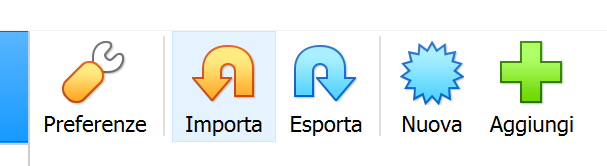
\includegraphics[width=0.4\textwidth]{../drawable/decorations/importing-button.png}
    \caption{The import button on the VirtualBox main page}
    \label{fig:getting-started:import-button}
\end{figure}

To follow, provide the \texttt{ova} file to VirtualBox and proceed to the next screen (Figure \ref{fig:getting-started:import-screen}). A long list will be shown. Please make sure that:

\begin{figure}[htbp]
	\centering
	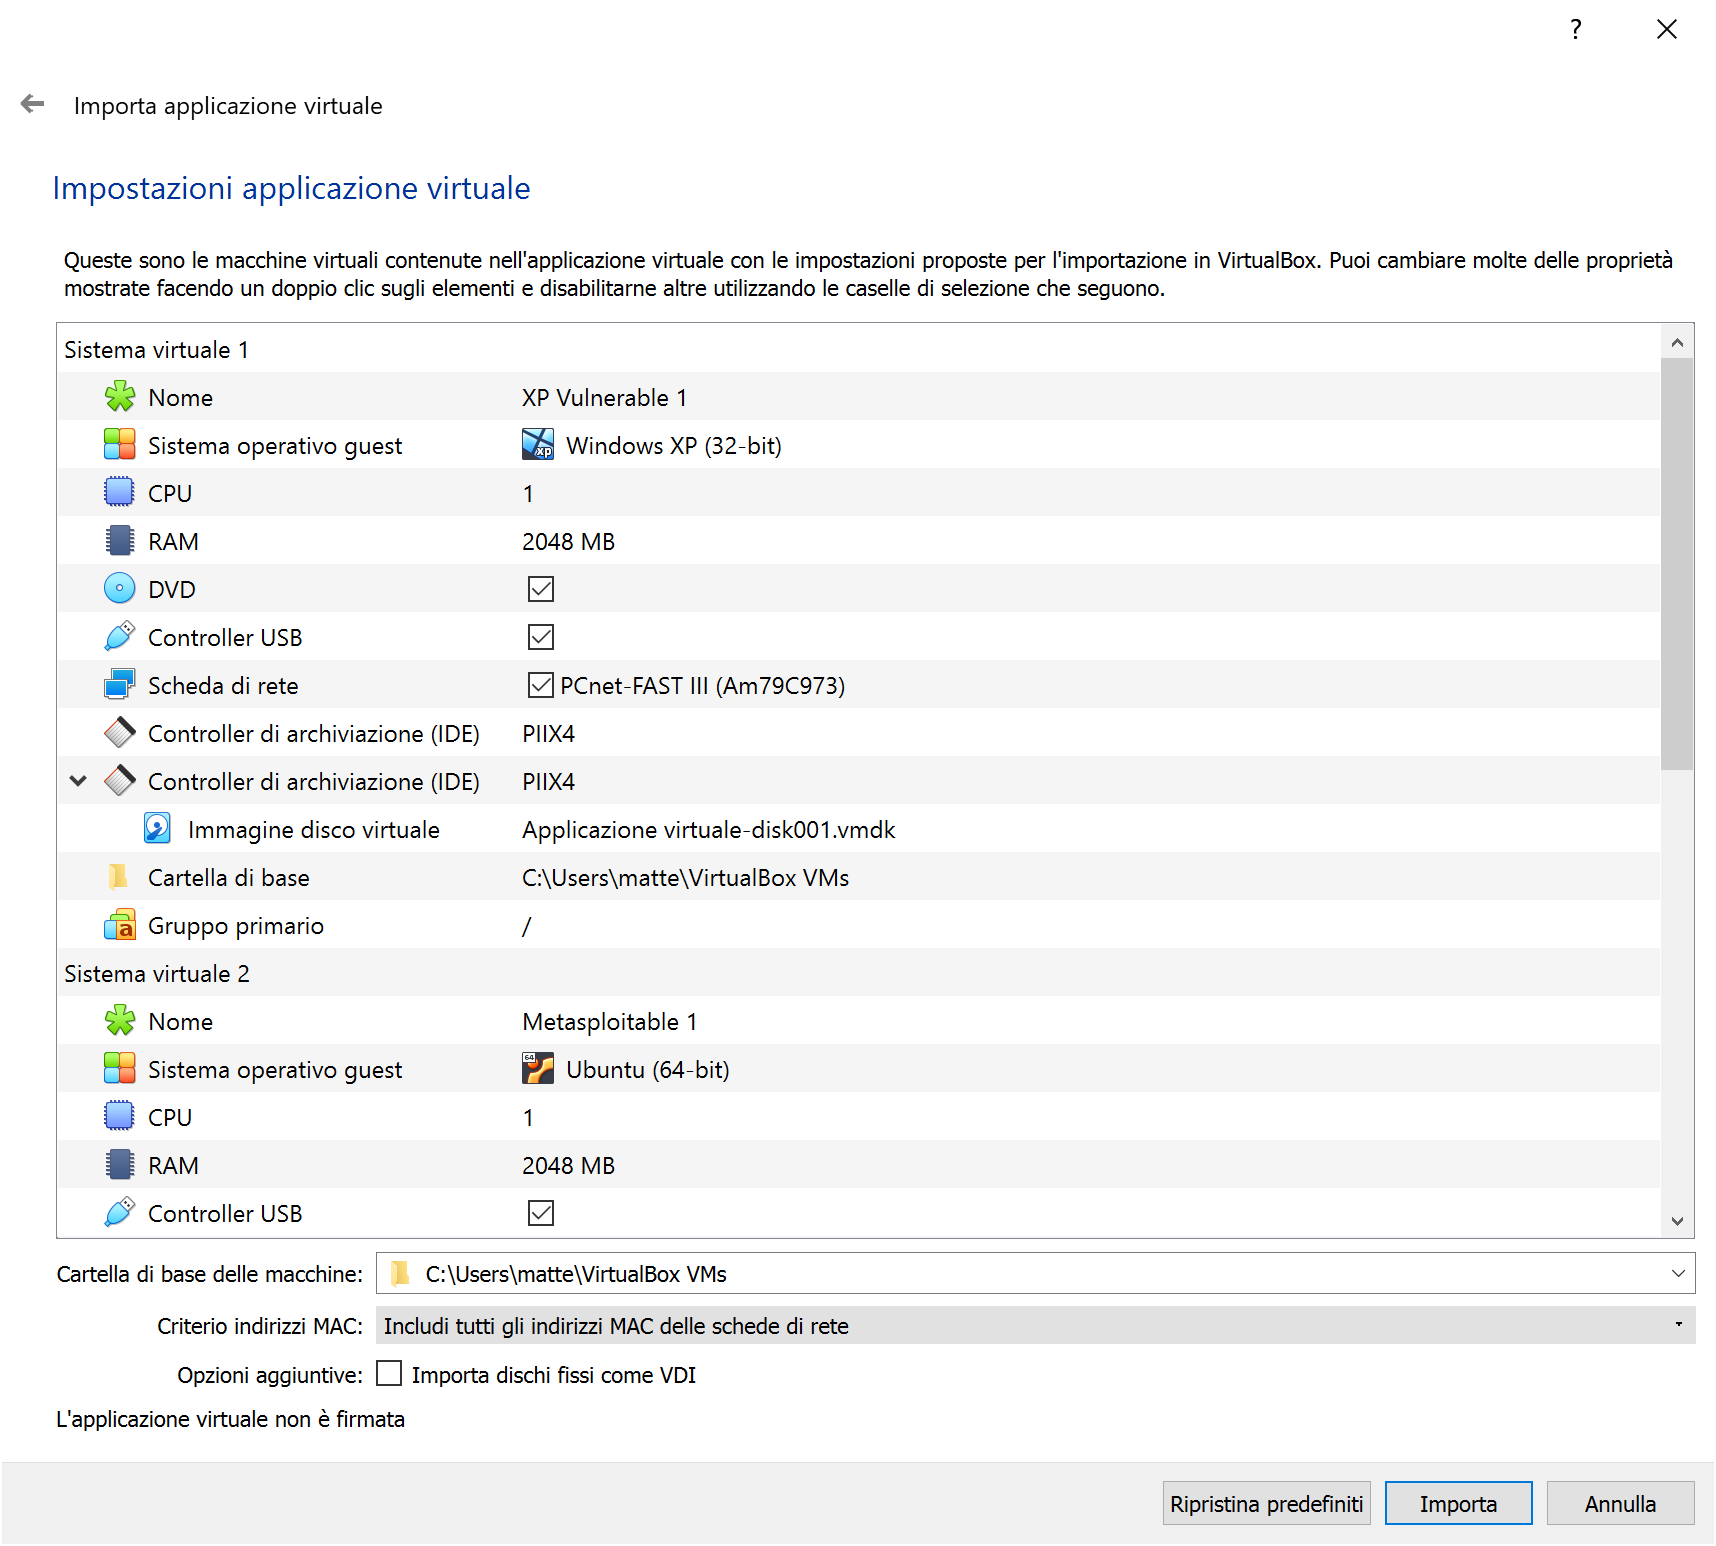
\includegraphics[width=0.7\textwidth]{../drawable/decorations/importing-screen.png}
    \caption{The final importing page}
    \label{fig:getting-started:import-screen}
\end{figure}

\begin{itemize}
    \item the MAC address dropdown menu is set to "Include all the MAC addresses"
    \item the saving location is set in a drive with at least \texttt{15 GB} of free space (\texttt{25 GB} recommended)
    \item there are three VMs to be imported: Windows XP, Metasploitable 1, Kali Linux-2021.1 1: the first two with 1 \texttt{vCPU}, the last with 2 \texttt{vCPU}, each one with \texttt{2048 MB} of RAM, a \texttt{vmdk} disk attached (with the USB controller set to on), and a network adapter.
\end{itemize}

If the requirements are unable to be satisfied by the host machine, you are free to reduce the RAM required by each machine by clicking it and editing it on the fly. Once the check is complete, please import the VMs and wait until all of them have been added to the list.

\subsubsection{Without the \texttt{ova} file}
\label{subsubsec:getting-started:without-ova}

The environment can be optionally recreated from scratch. First, VirtualBox must be installed along with the Oracle VM VirtualBox Extension Pack. Then, images for the three VMs must be retrieved and installed:

\begin{itemize}
    \item Kali Linux: downloadable from the offical website\footnote{\url{https://www.kali.org/downloads/}}
    \item Metasploitable 1: being a \texttt{EOL} product, can be retrieved from VulnHub\footnote{\url{https://www.vulnhub.com/entry/metasploitable-1,28/}}
    \item Windows XP: as it is not free software, it must be retrieved on one's own.
\end{itemize}

The Metasploitable machine is ready and does not need additional  modifications. The Windows XP machine is based on Windows XP SP2, and needs the following software to be installed:

\begin{itemize}
    \item \textbf{Adobe Reader} version \texttt{9.0.0} (to be used to execute the infected \texttt{PDF} exploit)
    \item \textbf{FreeSSHd} to offer \texttt{SSH} and \texttt{FTP} services (for remote management of the machine). The home directory for the \texttt{FTP} server has to be a shared folder.
    \item \textbf{Internet Information Services} installed (for the \texttt{TELNET} server)
\end{itemize}

The Kali Linux, depending on the flavor of the download, may or may not come with the Metasploit Framework installed, and additionally requires setting up the database. These steps can be found in Section \ref{subsec:getting-started:installing metasploit}.

Finally, remember to set up a virtual network bridge and to assign it to each VM's network interface in order to allow communication.

\subsection{Inspecting the environment}

Once the VMs are successfully deployed, we can proceed with the next step. First, start all of them and use the following credentials to log in once they have booted:

\begin{table}[htbp]
\centering
\begin{tabular}{|l|l|l|}
\hline 
Machine        & Username   & Password \\
\hline 
Kali Linux     & \texttt{kali}       & \texttt{kali}     \\
Metasploitable & \texttt{msfadmin}   & \texttt{msfadmin} \\
Windows XP     & \texttt{vulnerable} & \texttt{root}     \\
\hline
\end{tabular}
\end{table}

Then, open up a shell in each VM and verify the IPs (or set them, if you created them from scratch). They should be as in Figure \ref{fig:getting-started:network-conf}. Figure \ref{fig:getting-started:network-diagram} shows a simplified diagram of the obtained network.

\begin{figure}[htbp]
	\centering
	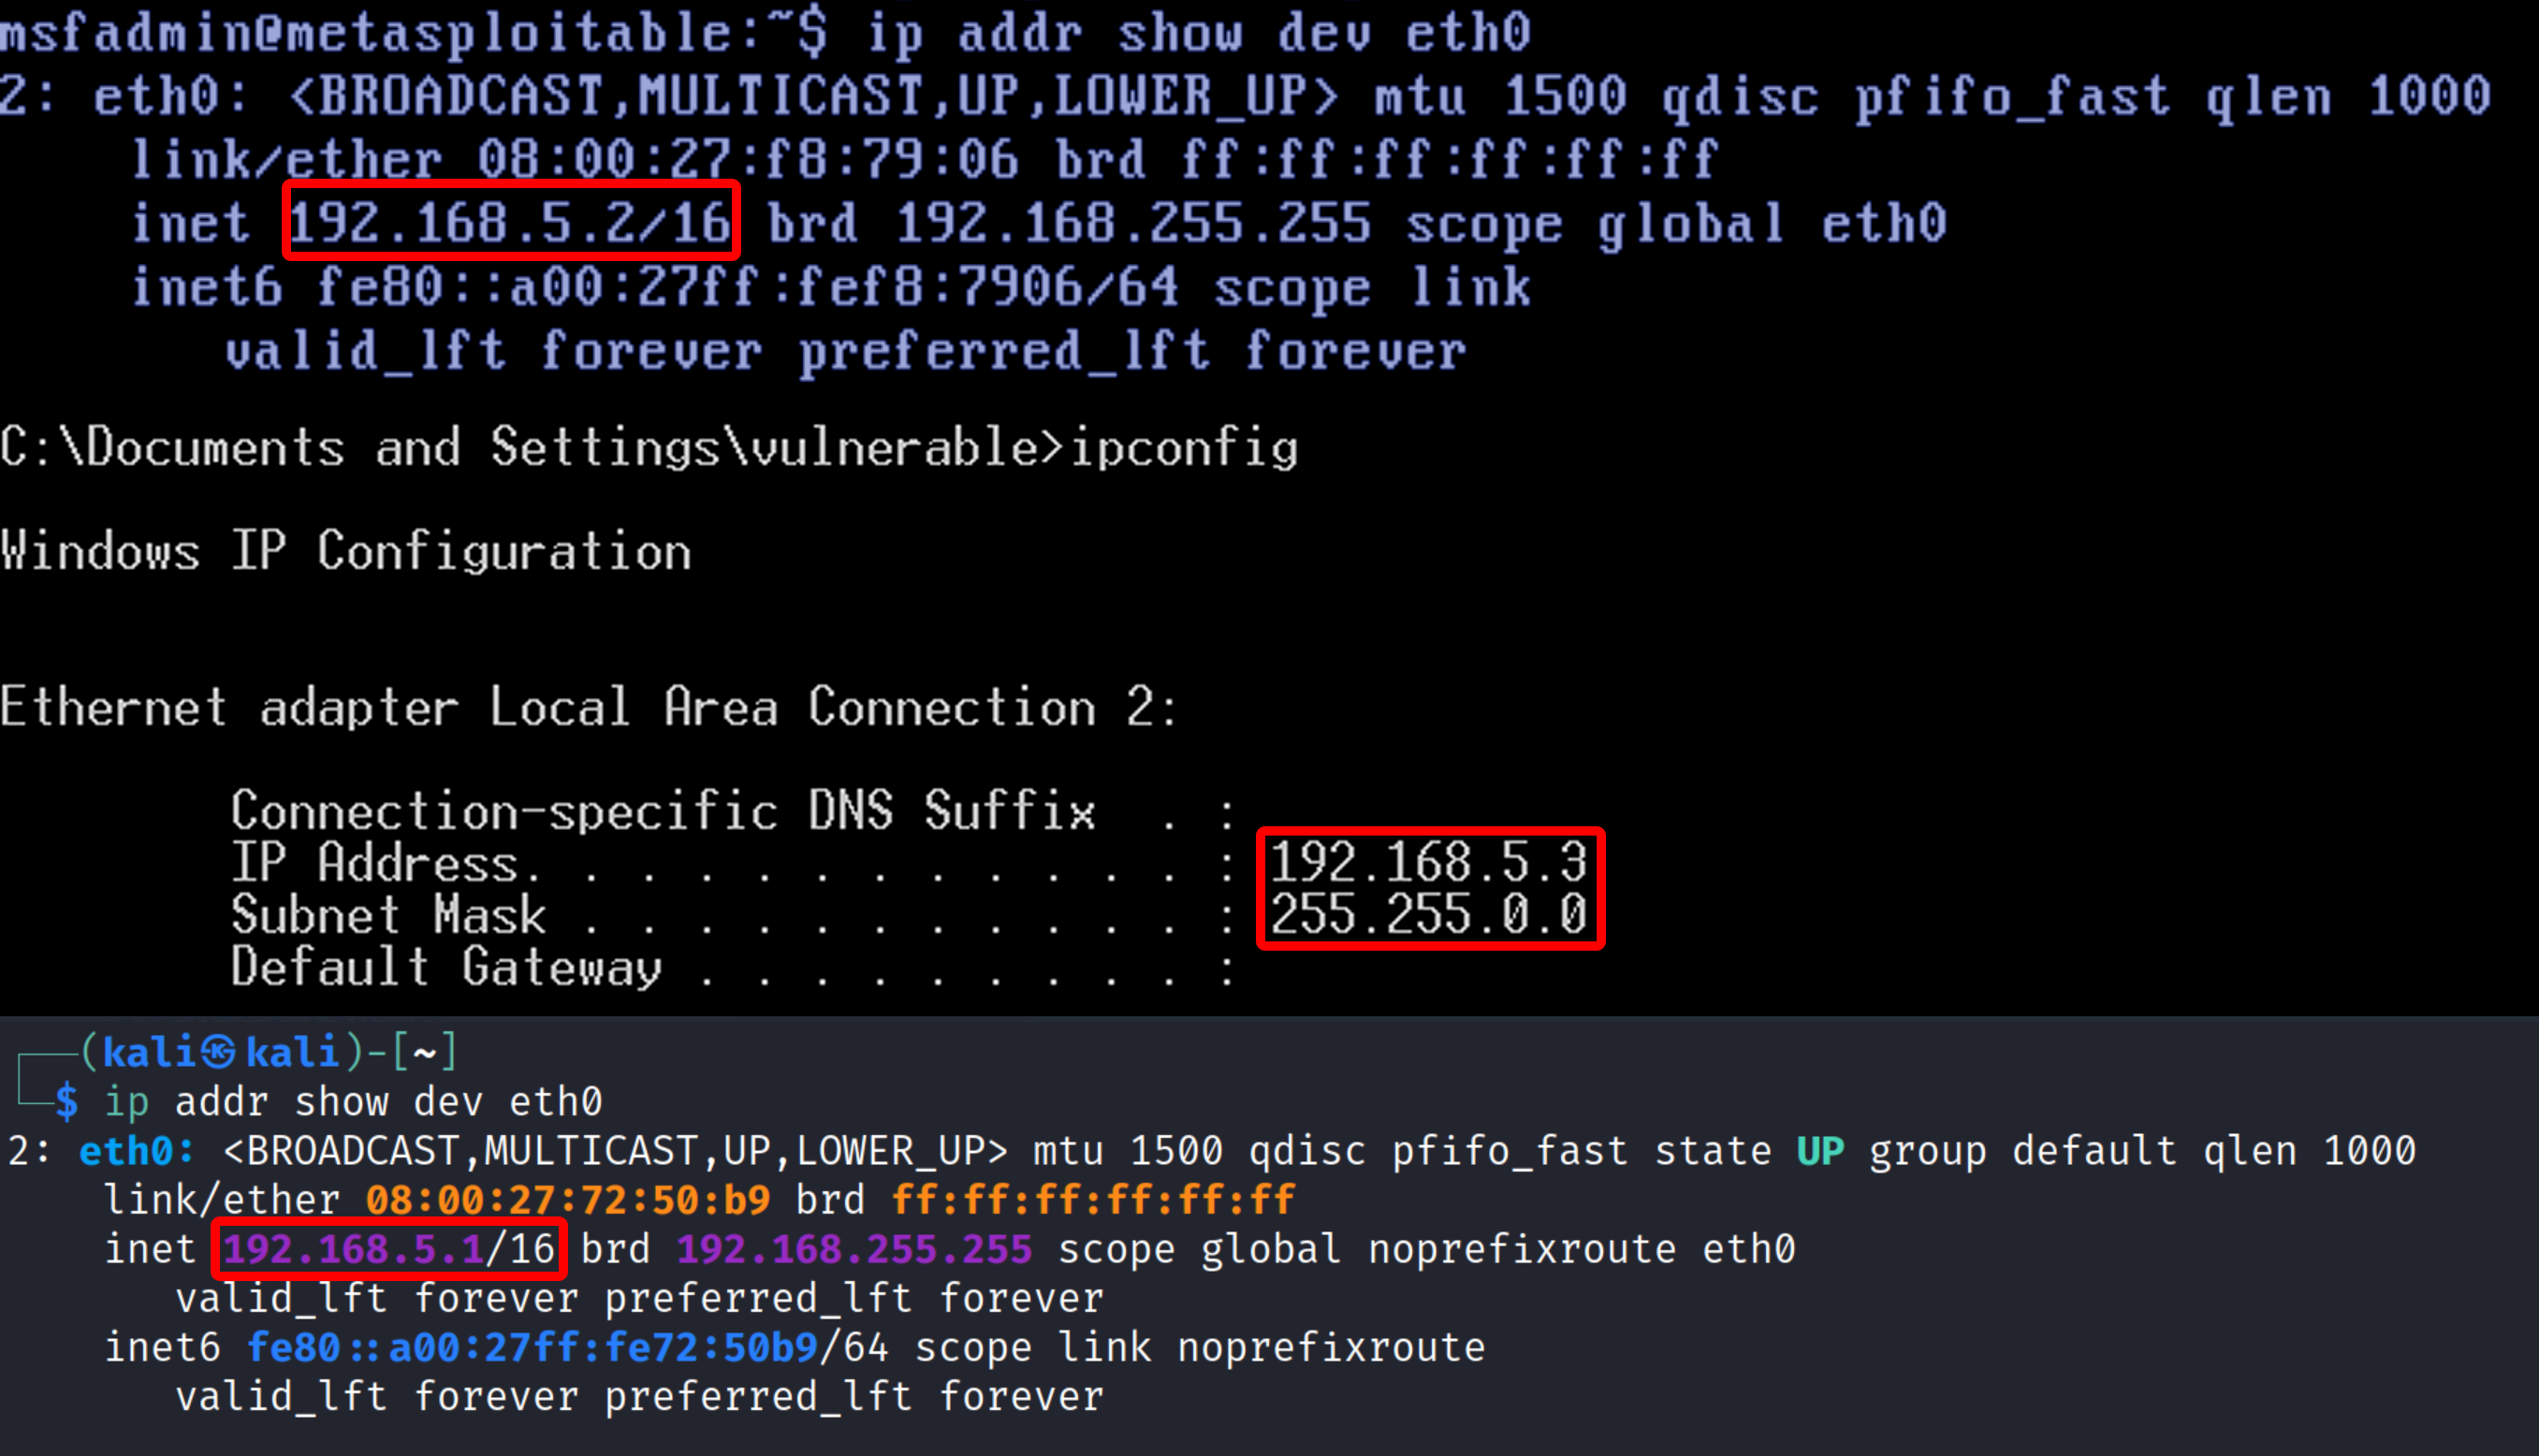
\includegraphics[width=\textwidth]{../drawable/preliminaries_screenshots/prel-ips.png}
    \caption{The network configuration for all VMs.}
    \label{fig:getting-started:network-conf}
\end{figure}

\begin{figure}[htbp]
	\centering
	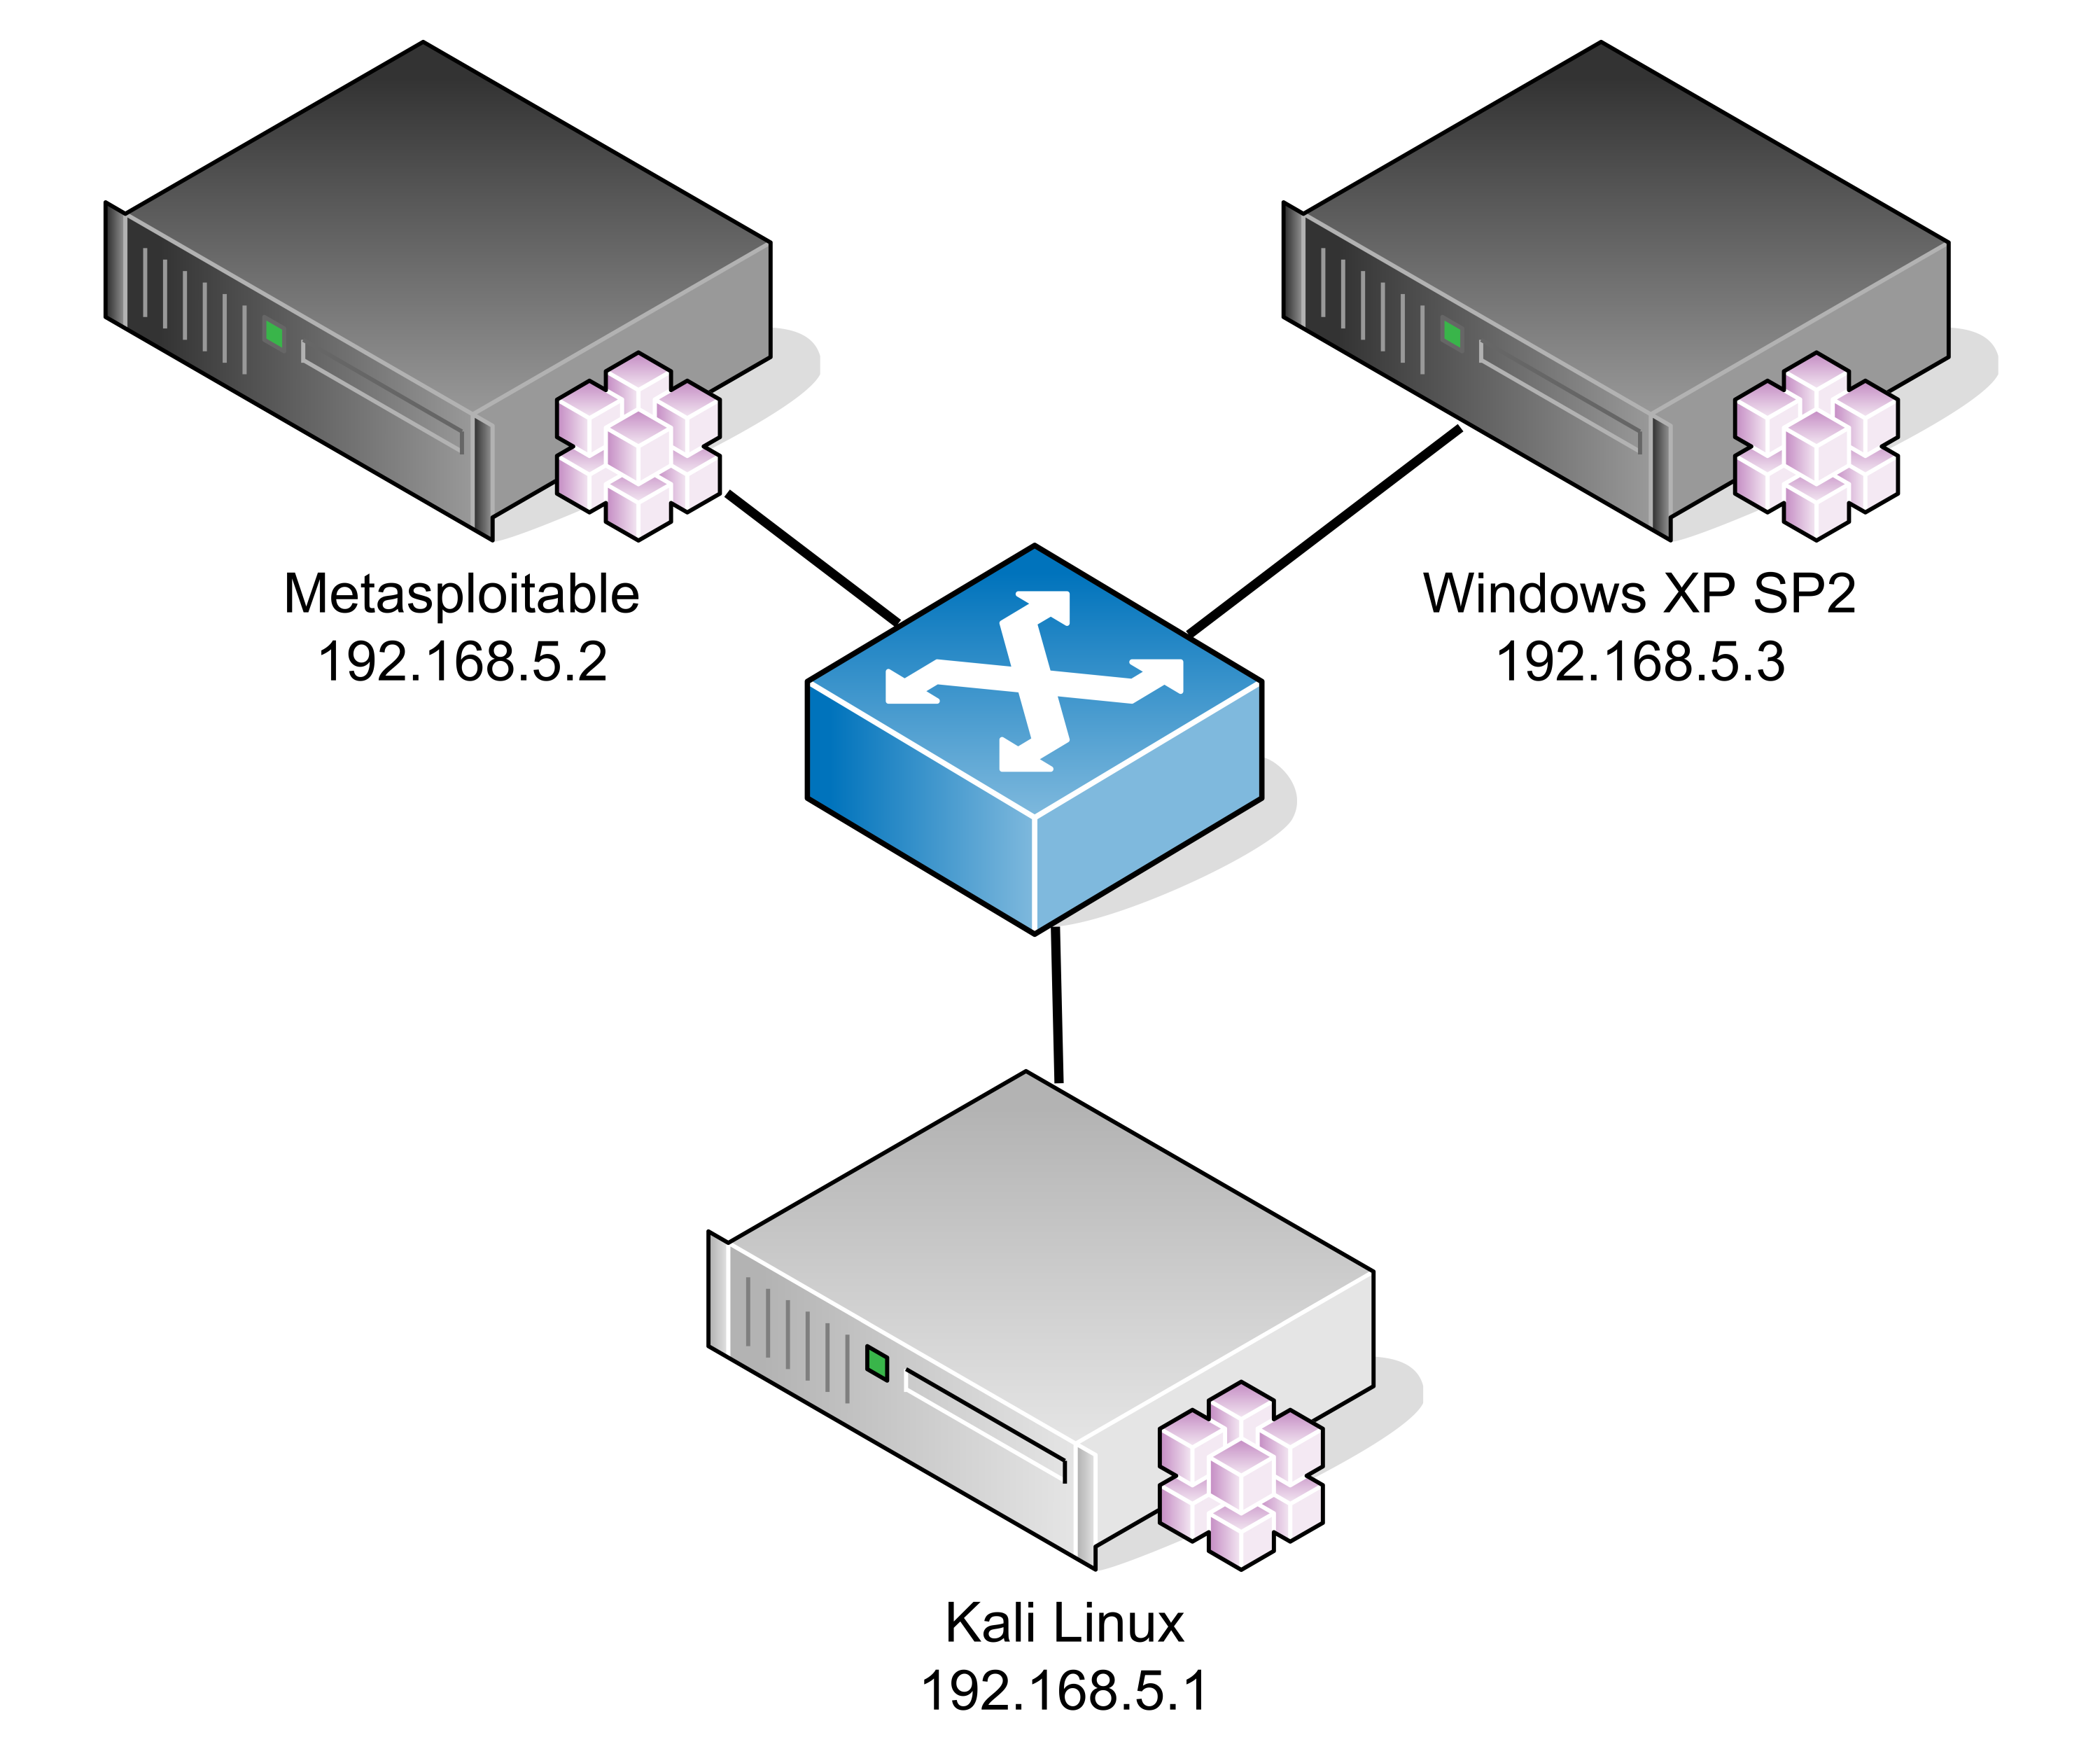
\includegraphics[width=0.4\textwidth]{../drawable/preliminaries_screenshots/prel-net.png}
    \caption{Diagram of the obtained network.}
    \label{fig:getting-started:network-diagram}
\end{figure}

\subsection{Installing Metasploit}
\label{subsec:getting-started:installing metasploit}

The following instructions are directly taken from the official Metasploit Framework page\footnote{\url{https://docs.rapid7.com/metasploit/installing-the-metasploit-framework/}}. Beginning from this section, code snippets shown in \hltexttt{dark\mbox{ }background} are intended as shell commands.\cite{online:msf-installation}

As Kali is a Linux distribution, we can proceed with the following command:

\begin{lstlisting}
curl "https://raw.githubusercontent.com/rapid7/metasploit-omnibus
    /master/config/templates/metasploit-framework-wrappers/
    msfupdate.erb" > msfinstall 
    && chmod 755 msfinstall 
    && ./msfinstall
\end{lstlisting}

We can then fire up \texttt{msfconsole}. Root privileges are recommended, as they will be needed in later exercises for both scanning and connection opening on well-known ports:

\begin{lstlisting}
sudo msfconsole
\end{lstlisting}

At startup, \texttt{msfconsole} will ask whether to set up a database. Insert \texttt{y} and let the console finalize the installation. If all goes well, inputting \texttt{db\_status} should yield:

\begin{lstlisting}
postgresql connected to msf
\end{lstlisting}

This means we're ready to get started with the basics of Metasploit.

\subsection{Commands}

The \texttt{msfconsole} is a full fledged shell with autocompletion and help pages. Inserting \hltexttt{?} or \hltexttt{help} will yield a long help page which covers all commands available for the user. For now, we will however focus on navigation and very basic usage.

As we said before, Metasploit's functionalities are logically divided into modules. \texttt{msfconsole} is packed with a powerful search tool which can index and retrieve modules very efficiently. To get started, one can write

\begin{lstlisting}
search eternalblue
\end{lstlisting}

in order to retrieve a full list of results of modules related to our query:

\begin{figure}[htbp]
	\centering
	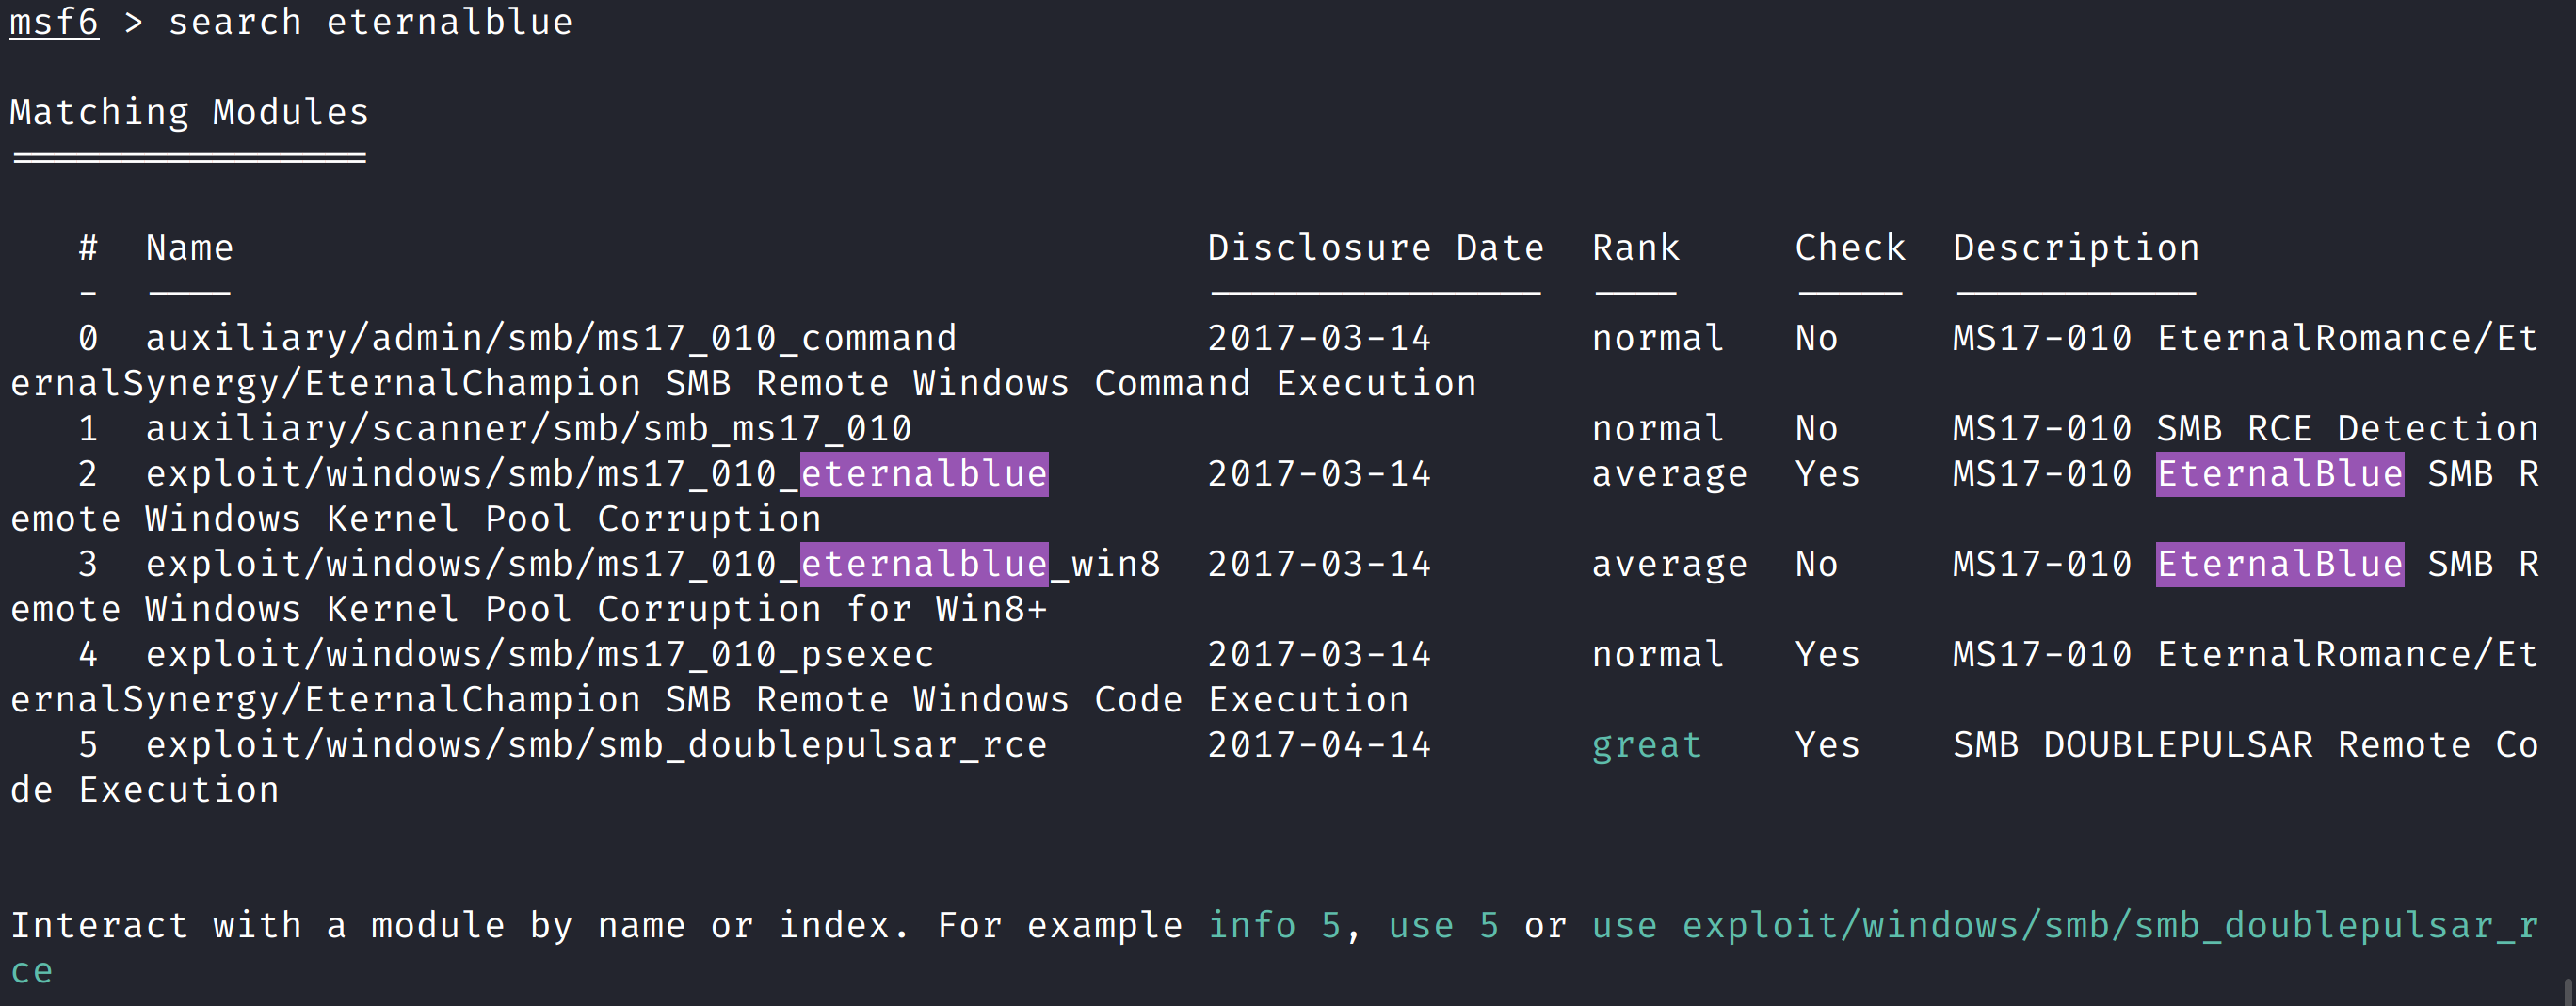
\includegraphics[width=\textwidth]{../drawable/preliminaries_screenshots/search-eternalblue.png}
    \caption{The results of a query in \texttt{msfconsole}}
    \label{fig:getting-started:query-search}
\end{figure}

Each module is sorted hierarchically by type, then platform, and then protocol. For example, we can inspect the infamous DoublePulsar exploit (listed as \texttt{exploit/windows/smb/smb\_doublepulsar\_rce}) by typing \hltexttt{info\mbox{ }5} - the index in the newly printed list - or just typing \hltexttt{info} followed by the module name. The console comes into help with autocompletion by tabbing.

Other important values shown and not shown in the table include:

\begin{itemize}
    \item the disclosure date (\texttt{date})
    \item the ranking (\texttt{ranking}), which provides details about the reliability and impact of an exploit on a target (ranging from Low to Excellent)
    \item the affected platform (\texttt{platform})
    \item the type (\texttt{type})
    \item the CVE ID if present (\texttt{cve})
\end{itemize}

Each of these values can be used against the search against in order to narrow down a search:

\begin{lstlisting}
search platform:windows description:acrobat
search cve:2021 type:exploit
search type:payload 
\end{lstlisting}

The amount of filters is vast. Typing \hltexttt{help\mbox{ }search} will provide more than adequate information for the matter.

Once a module has been selected, we can move into the next phase by typing \hltexttt{use} followed by the search index number or the name. The shell will react accordingly, switching modes (Figure \ref{fig:getting-started:using-module}).

\begin{figure}[htbp]
	\centering
	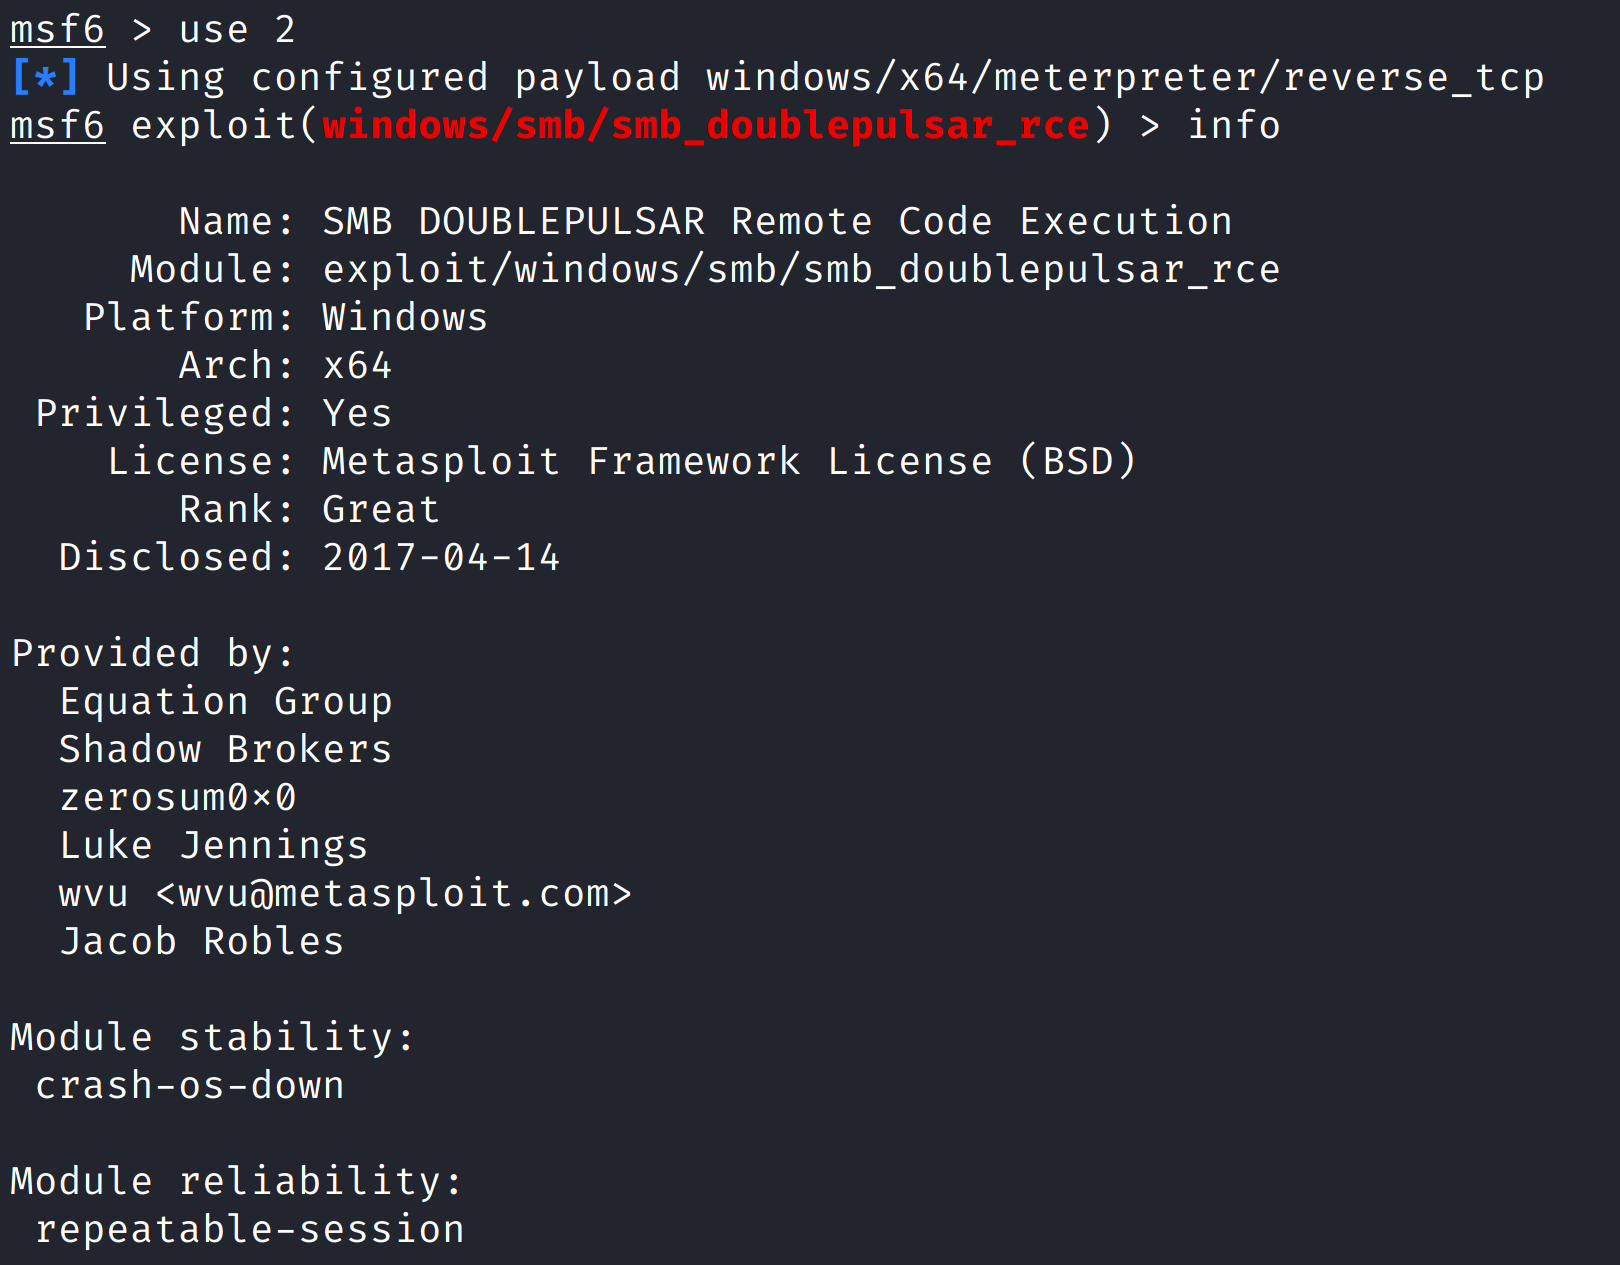
\includegraphics[width=0.7\textwidth]{../drawable/preliminaries_screenshots/info-eternalblue.png}
    \caption{Using a module in \texttt{msfconsole}: first, the mode switch, then an \hltexttt{info} command showing some information}
    \label{fig:getting-started:using-module}
\end{figure}

In this mode, we can type \hltexttt{info} to get a detailed report of the module at any time. Figure \ref{fig:getting-started:using-module} shows a small portion of the information about the DoublePulsar exploit we have chosen. Additionally, we can notice that when we typed \hltexttt{use\mbox{ }2} the Framework reminded us that the pre-configured payload was loaded (\texttt{windows/x64/meterpreter/reverse\_tcp}). Each exploit module has usually a default payload: we can surely change it with the following commands:

\begin{lstlisting}
show payloads
set payload [...]
\end{lstlisting}

It must be reminded that payloads are to be set only in case of exploit modules. In either case, we can have a glance at all the options of the module with \hltexttt{show\mbox{ }options}. Each one of them can be then \hltexttt{set} or \hltexttt{\mbox{unset}} with the homonymous commands.

\begin{figure}[htbp]
	\centering
	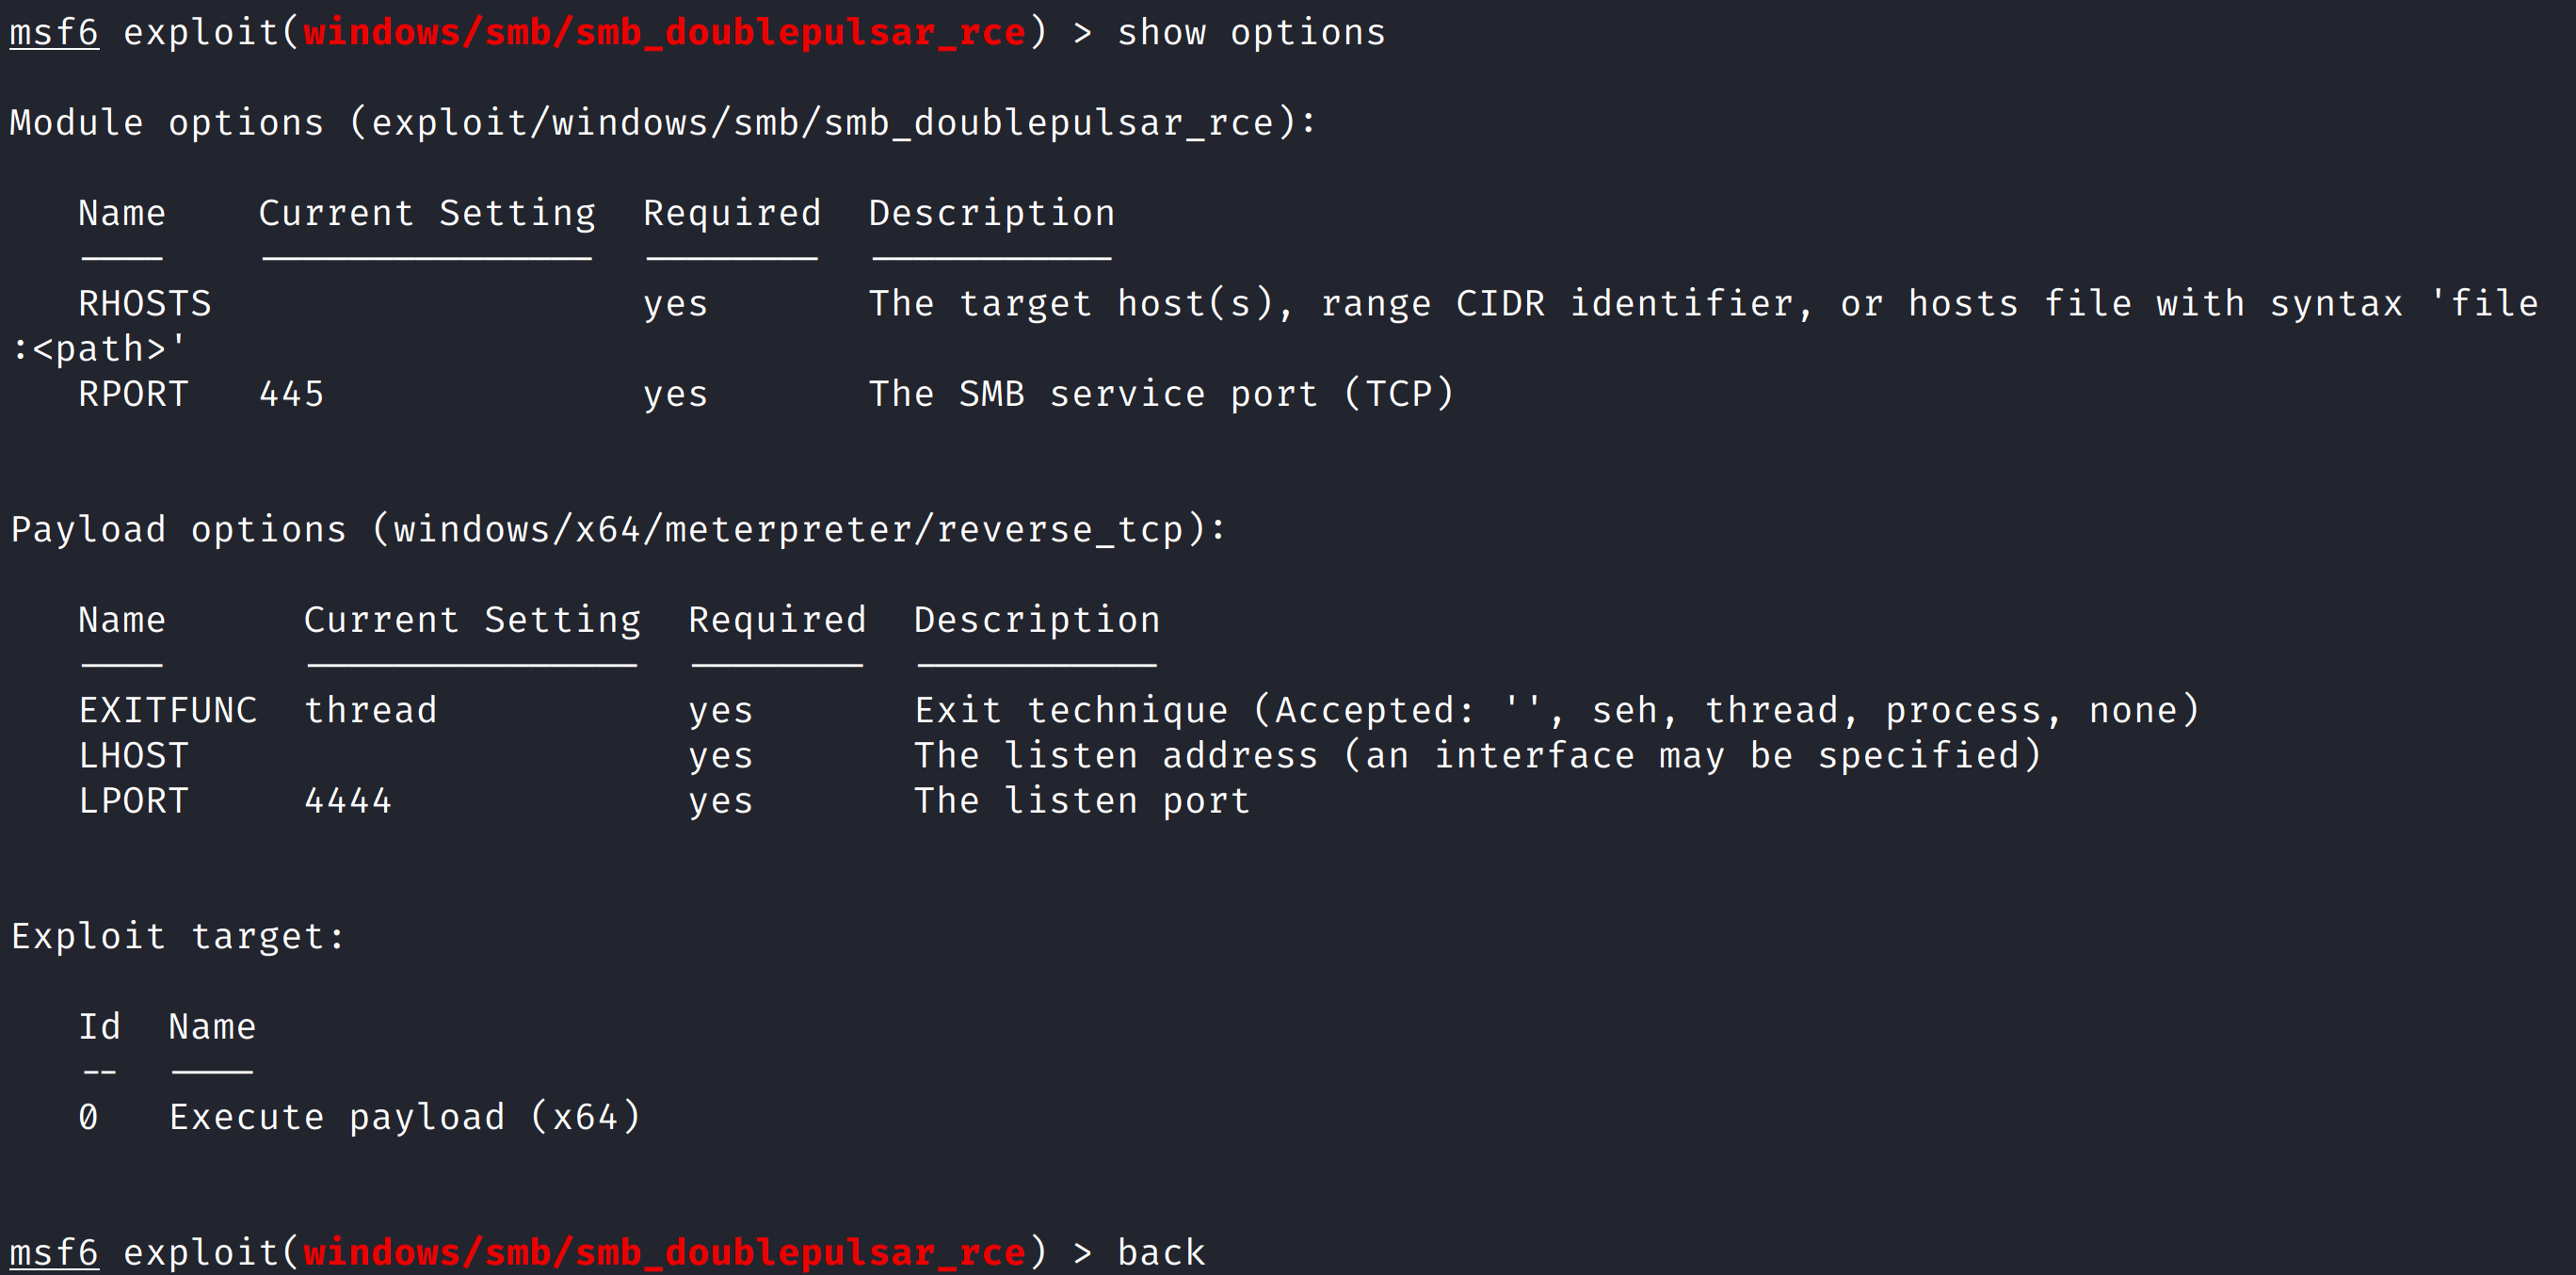
\includegraphics[width=\textwidth]{../drawable/preliminaries_screenshots/options-eternalblue.png}
    \caption{Showing a module's options, and going \hltexttt{back}}
    \label{fig:getting-started:options-back}
\end{figure}


Once we're set, we can mount the attack (in case of an exploit) with the \hltexttt{\mbox{exploit}} command, or run the module with \hltexttt{run}. For now, however, we'll just go \hltexttt{back} once to the main menu (Figure \ref{fig:getting-started:options-back}).

We conclude this introduction with a quick look at some supplementary commands:

\begin{itemize}
    \item \hltexttt{edit} - brings up the system textedit program to edit a particular file or, if run within a module, the module itself.
    \item \hltexttt{grep} - works exactly as its Unix counterpart (Warning! Pipes do not work within \texttt{msfconsole}. Use \texttt{grep} followed by the required command).
    \item \hltexttt{irb} - starts a Ruby shell, within the context of the current module.
    \item \hltexttt{jobs} - lists active jobs such as ongoing exploits.
    \item \hltexttt{kill} - shuts down an ongoing activity.
    \item \hltexttt{\mbox{sessions}} - shows currently open connections. Will be used in later exercises.
\end{itemize}

\clearpage
\section{Exercise 1}
\label{sec:exercise1}

The first exercise's objective is to take a grasp's Metasploit's \texttt{auxiliary} library and to use it for some simple reconnaissance tasks on the network.

Metasploit is packed with a deep auxiliary library, called the Metasploit \textit{EXploitation} library (and known as \texttt{lib}\texttt{/msf}\texttt{/core} within the Ruby source code). Its objective is to automate as much as possible typical reconnaissance tasks.

The auxiliary library provides a lot of tools. They include server capture modules (for sniffing credentials or collecting password hashes), scanners (of all sorts: TCP, UDP, HTTP, etc...), and administrative modules (for directory listing, identification of admin panels, and more), fuzzers, brute forcers, and even DoS managers.

\subsection{TCP scanning}
\label{sec:exercise1:tcpscanning}

Let us start by examining open some ports on our targets. We can either use \texttt{Nmap} or one of the auxiliary Metasploit modules. We'll defer the use of the former to the next exercise, which will also employ Metasploit's database. For now, let's load the TCP scanner module and run it against the whole subnet.\cite{online:msf-scanning-enumeration}\cite{online:msf-auxmodules}

\begin{lstlisting}
use auxiliary/scanner/portscan/tcp
\end{lstlisting}

\begin{figure}[htbp]
	\centering
	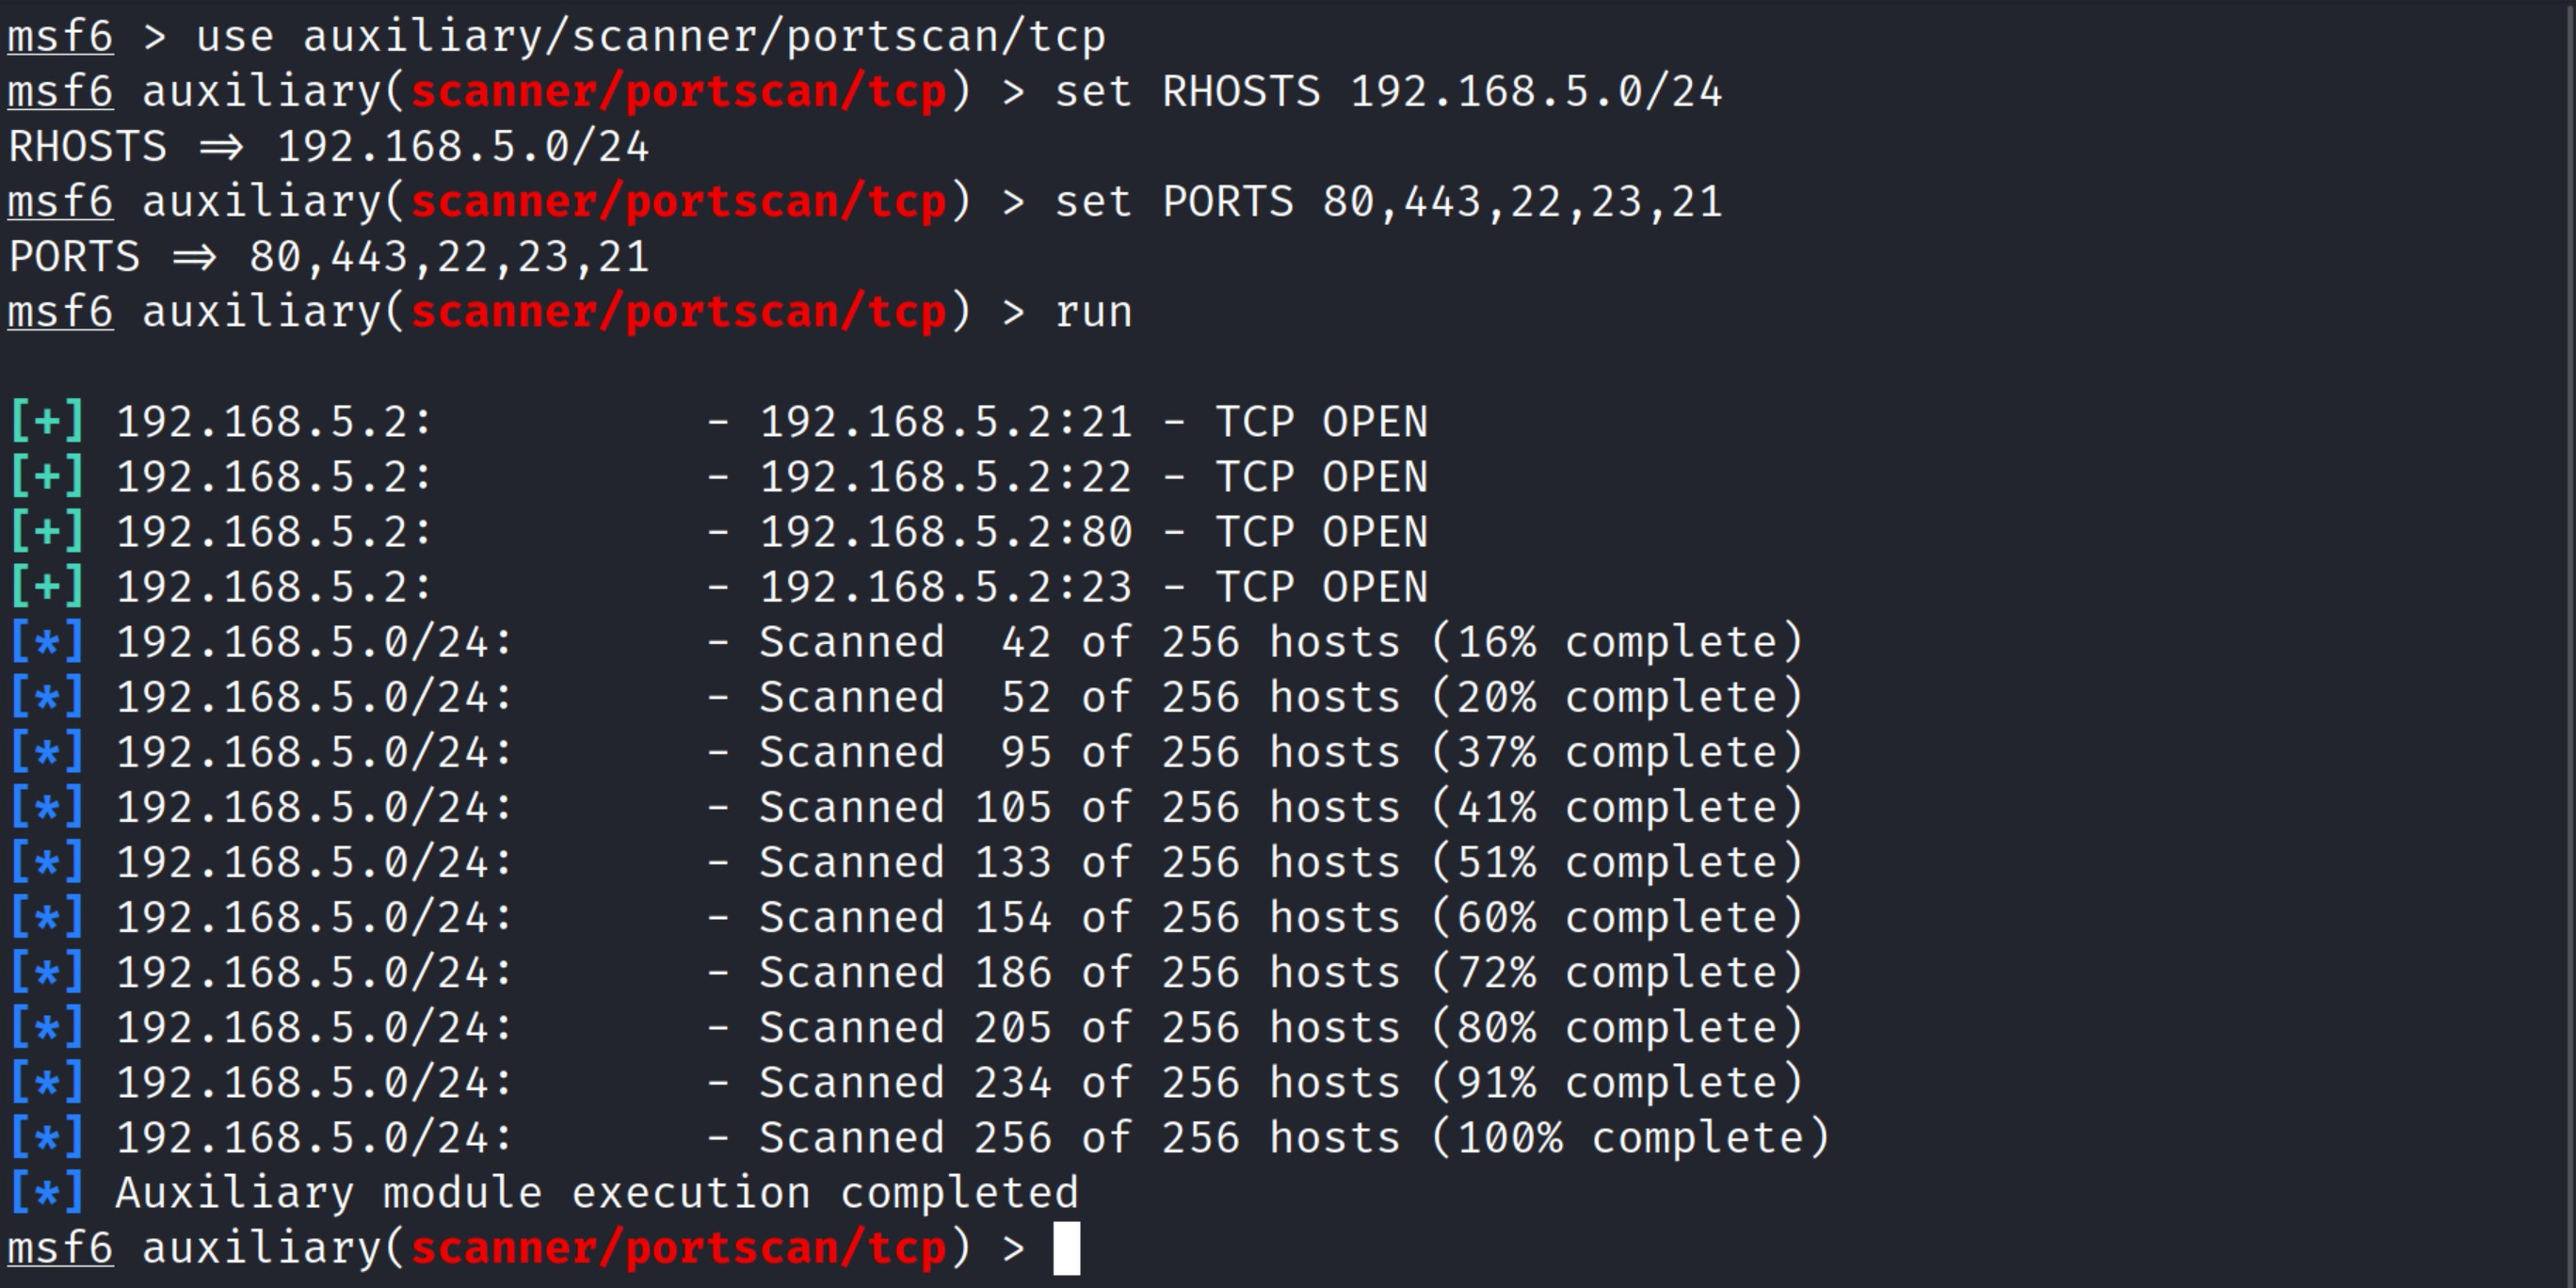
\includegraphics[width=0.9\textwidth]{../drawable/exercise_1_screenshots/es1-scan.jpg}
	\caption{Setting options for the \texttt{TCP} scanner and running it}
	\label{fig:ex1:scan}
\end{figure}

Metasploit still provides various scanners, such as a \texttt{SYN} one. Additionally, we deliberately inserted a few ports in this example just to showcase the usage of the tool. In Section \ref{sec:ex2} a more accurate and complete scan will be executed.

\subsection{SSH scanning and brute forcing}

Next, we show an example of \texttt{SSH} server scanning and brute forcing. We just verified with the TCP scanner that the Metasploitable machine is exposing an \texttt{SSH} server on port 22. Let us fingerprint the version first. We load the following module:

\begin{lstlisting}
use auxiliary/scanner/ssh/ssh_version
\end{lstlisting}

We \hltexttt{set} the \texttt{RHOSTS} variable and \hltexttt{run} it. Figure \ref{fig:ex1:ssh} shows the output of this command.

\begin{figure}[htbp]
	\centering
	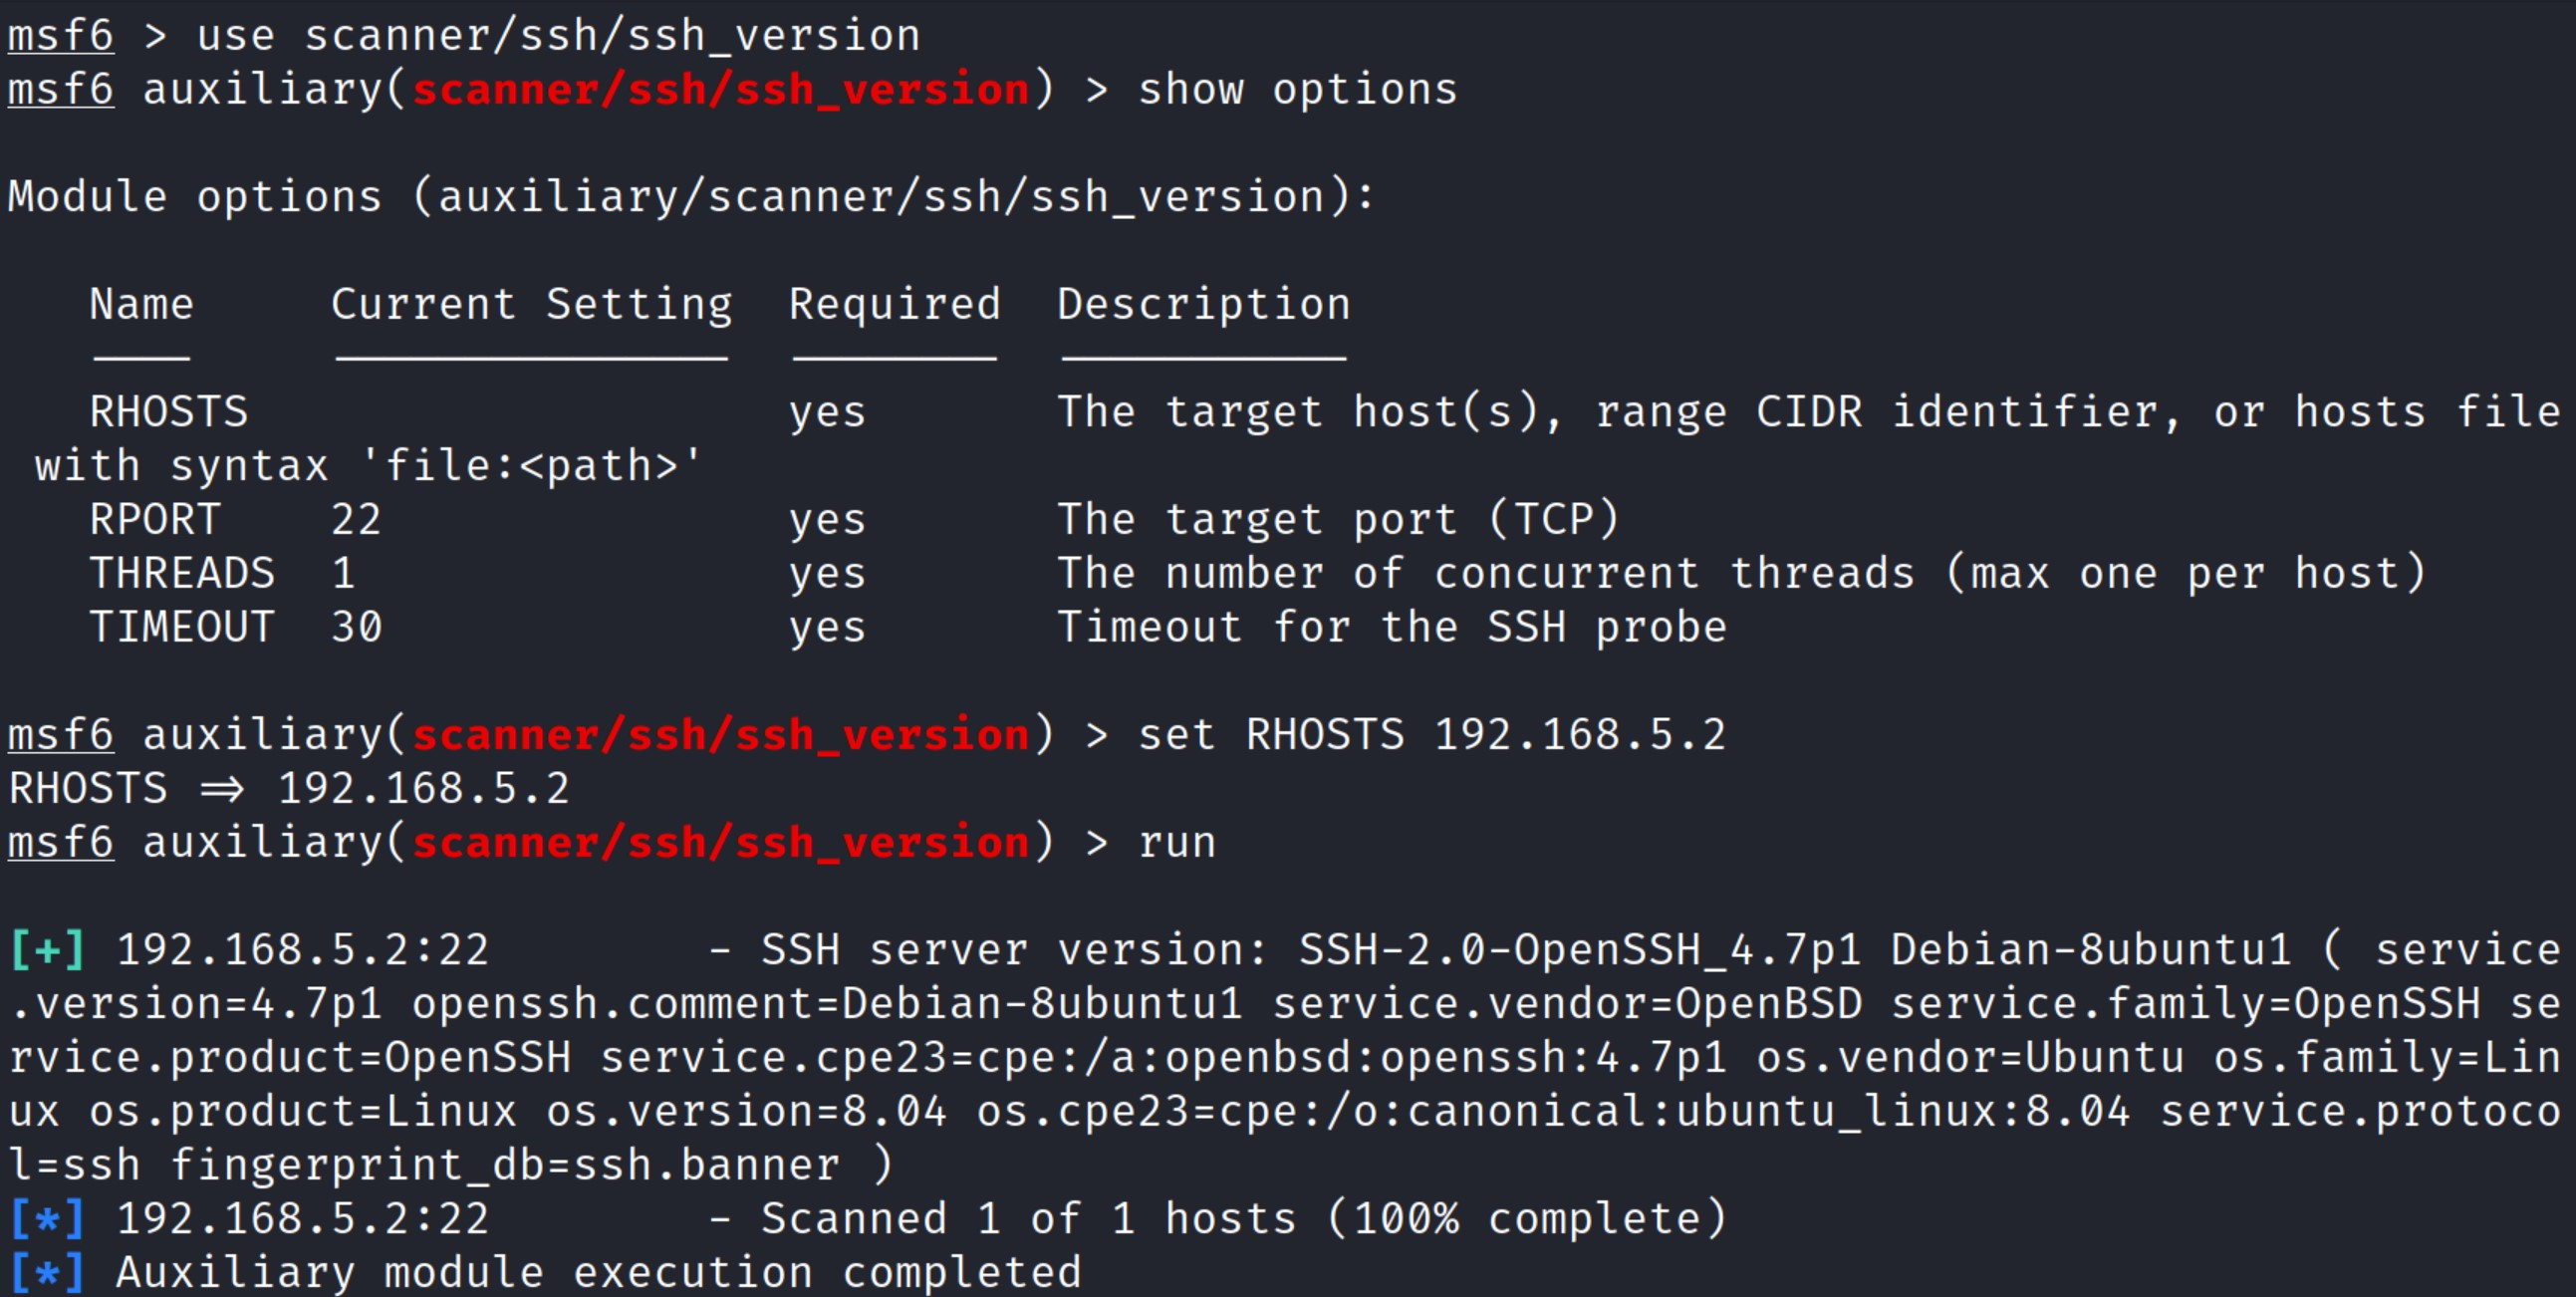
\includegraphics[width=\textwidth]{../drawable/exercise_1_screenshots/es1-ssh.jpg}
	\caption{Scanning the \texttt{SSH} version.}
	\label{fig:ex1:ssh}
\end{figure}

On first sight, it looks an innocent OpenSSH server running on top of a very old Ubuntu version. We can try the good old-fashioned way and mount a brute force attack with a dictionary file to see whether we can take over the machine without resorting to other exploits. We load the following module:

\begin{lstlisting}
use auxiliary/scanner/ssh/ssh_login
\end{lstlisting}

First, we \hltexttt{set} the \texttt{RHOSTS} variable as usual, but this time we also employ a file, called \texttt{passwords.txt} and saved in the home directory of Kali, and we \hltexttt{set} it against the \texttt{USERPASS\_FILE} variable. We can inspect the file on a separate shell:

\begin{lstlisting}
---(kali@kali)-[~]
--$ cat passwords.txt 

user password
msfadmin msfadmin
user user
root user
root password
\end{lstlisting}

For the purposes of this exercise, we inserted a handful of passwords just to show the mechanism of the module. Real life userpass files contain thousands of thousands of username and password combinations. Once the module has been executed, we should have obtained two shell logins. Figure \ref{fig:ex1:brutessh} shows the output of the module.

\begin{figure}[htbp]
	\centering
	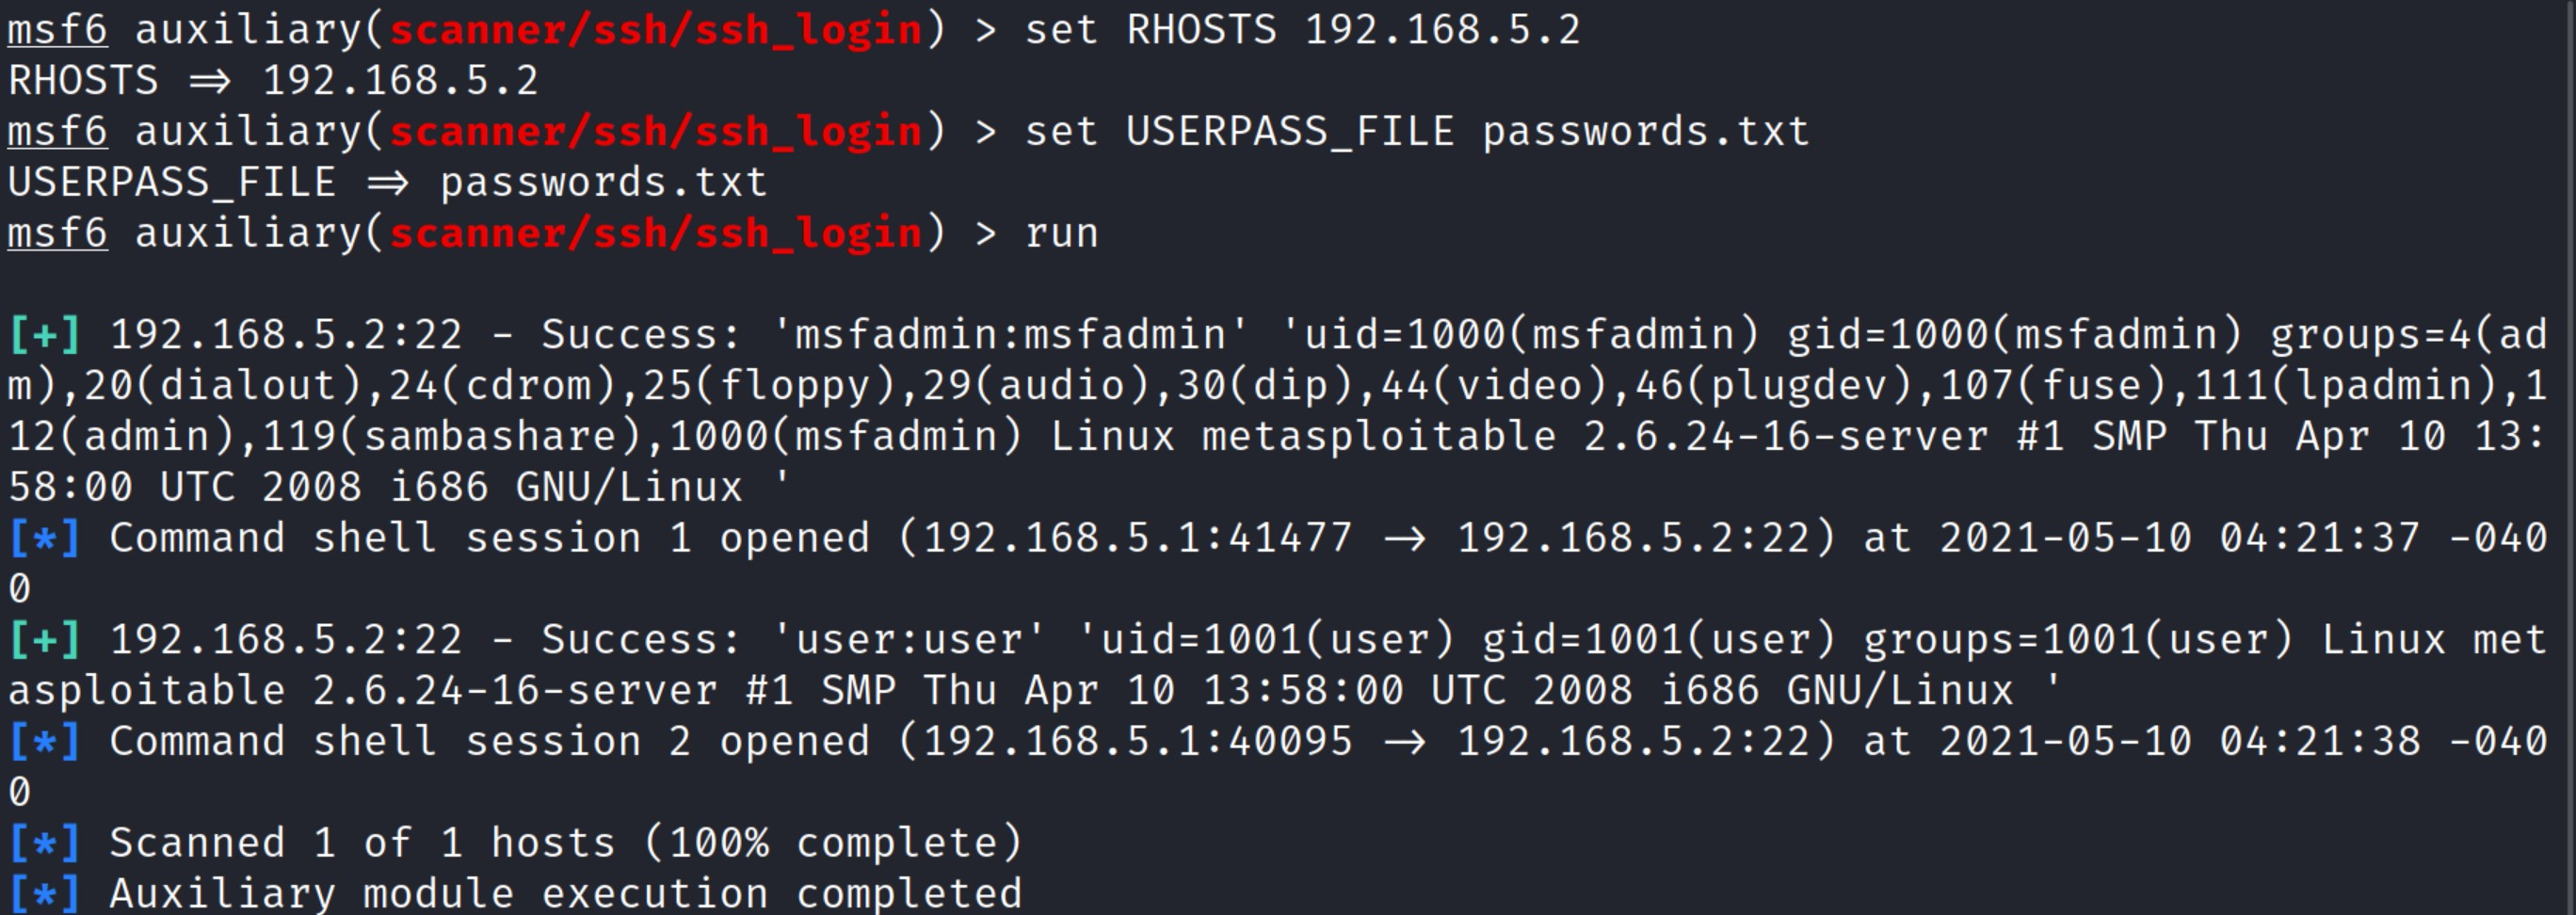
\includegraphics[width=\textwidth]{../drawable/exercise_1_screenshots/es1-brutessh.jpg}
	\caption{Taking over the \texttt{SSH} webserver with an userpass file.}
	\label{fig:ex1:brutessh}
\end{figure}

This time, we intentionally inserted two valid username and password combinations in the \texttt{passwords.txt} file. One of them (\texttt{msfadmin}, \texttt{msfadmin}) opened a full, root-privileged shell. The other one (\texttt{user}, \texttt{user}) opened a regular one. In fact, we can derive that from Figure \ref{fig:ex1:brutessh}, in which the first username/password hit shows \texttt{gid=1000(msfadmin)}, while the second one shows \texttt{gid=1001(user)}.

This resulted in two open connections. We can check the active sessions with the \hltexttt{\mbox{sessions}} command. Figure \ref{fig:ex1:sshsessions} shows the output of the command.

\begin{figure}[htbp]
	\centering
	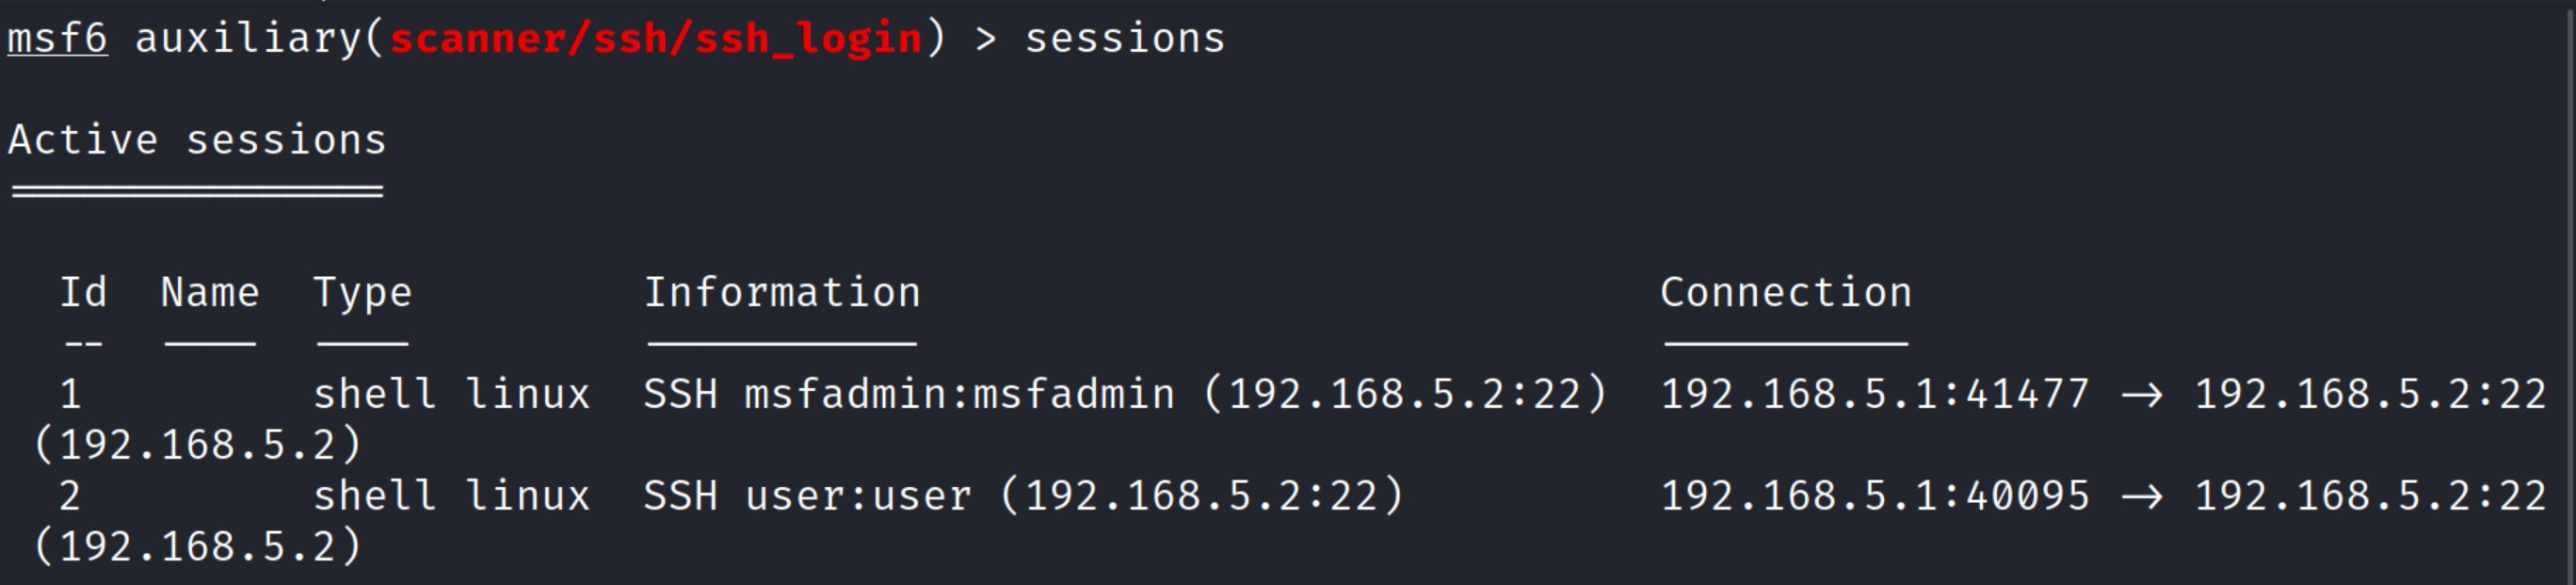
\includegraphics[width=\textwidth]{../drawable/exercise_1_screenshots/es1-sshsessions.jpg}
	\caption{The active sessions.}
	\label{fig:ex1:sshsessions}
\end{figure}

\subsection{HTTP scanning}
The amount of modules is vast. We conclude this exercise by checking the running version of a web server and listing its available directories. The following modules come into play:

\begin{lstlisting}
use auxiliary/scanner/http/http_version
use auxiliary/scanner/http/dir_scanner
\end{lstlisting}

Both modules require setting the \texttt{RHOSTS} variable to a corresponding target. We will just target the Metasploitable machine (bound on the \texttt{.2} IP address) as the XP one is not interesting in this case and has no open web server. 

\begin{figure}[htbp]
	\centering
	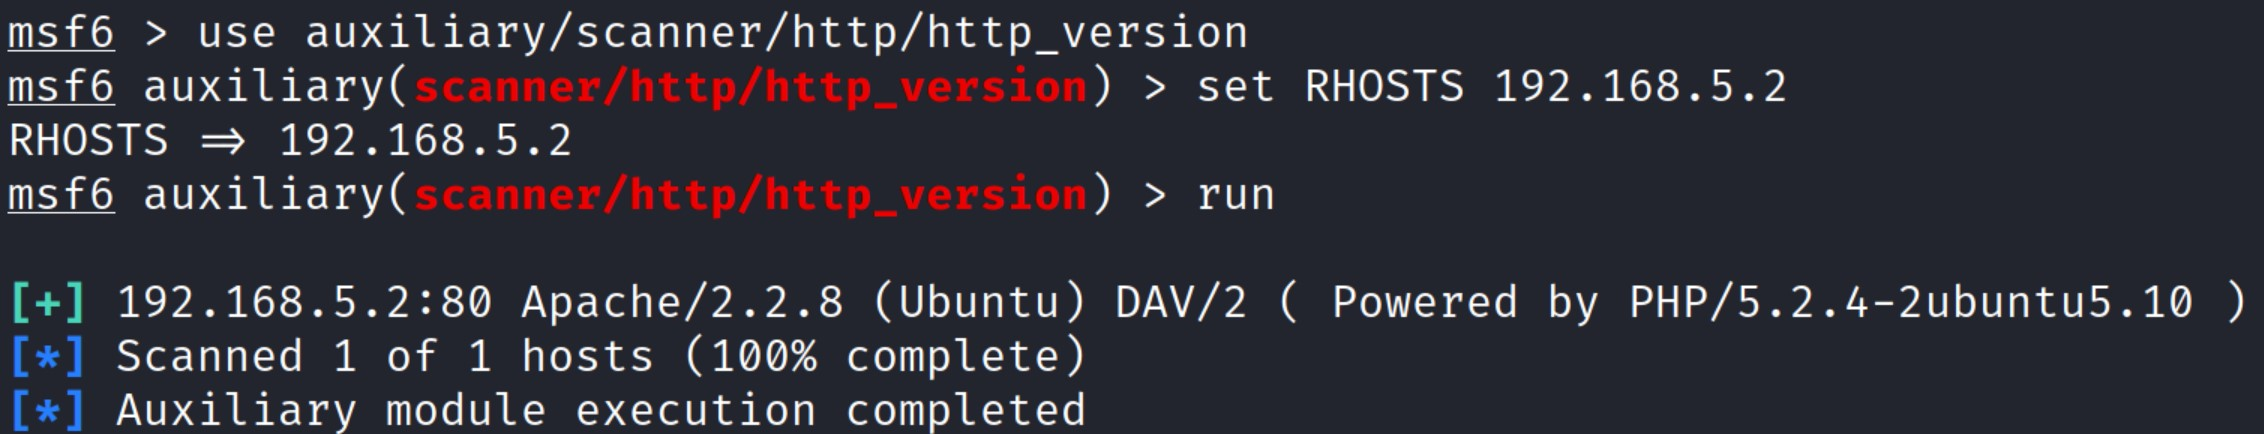
\includegraphics[width=\textwidth]{../drawable/exercise_1_screenshots/es1-http.jpg}
	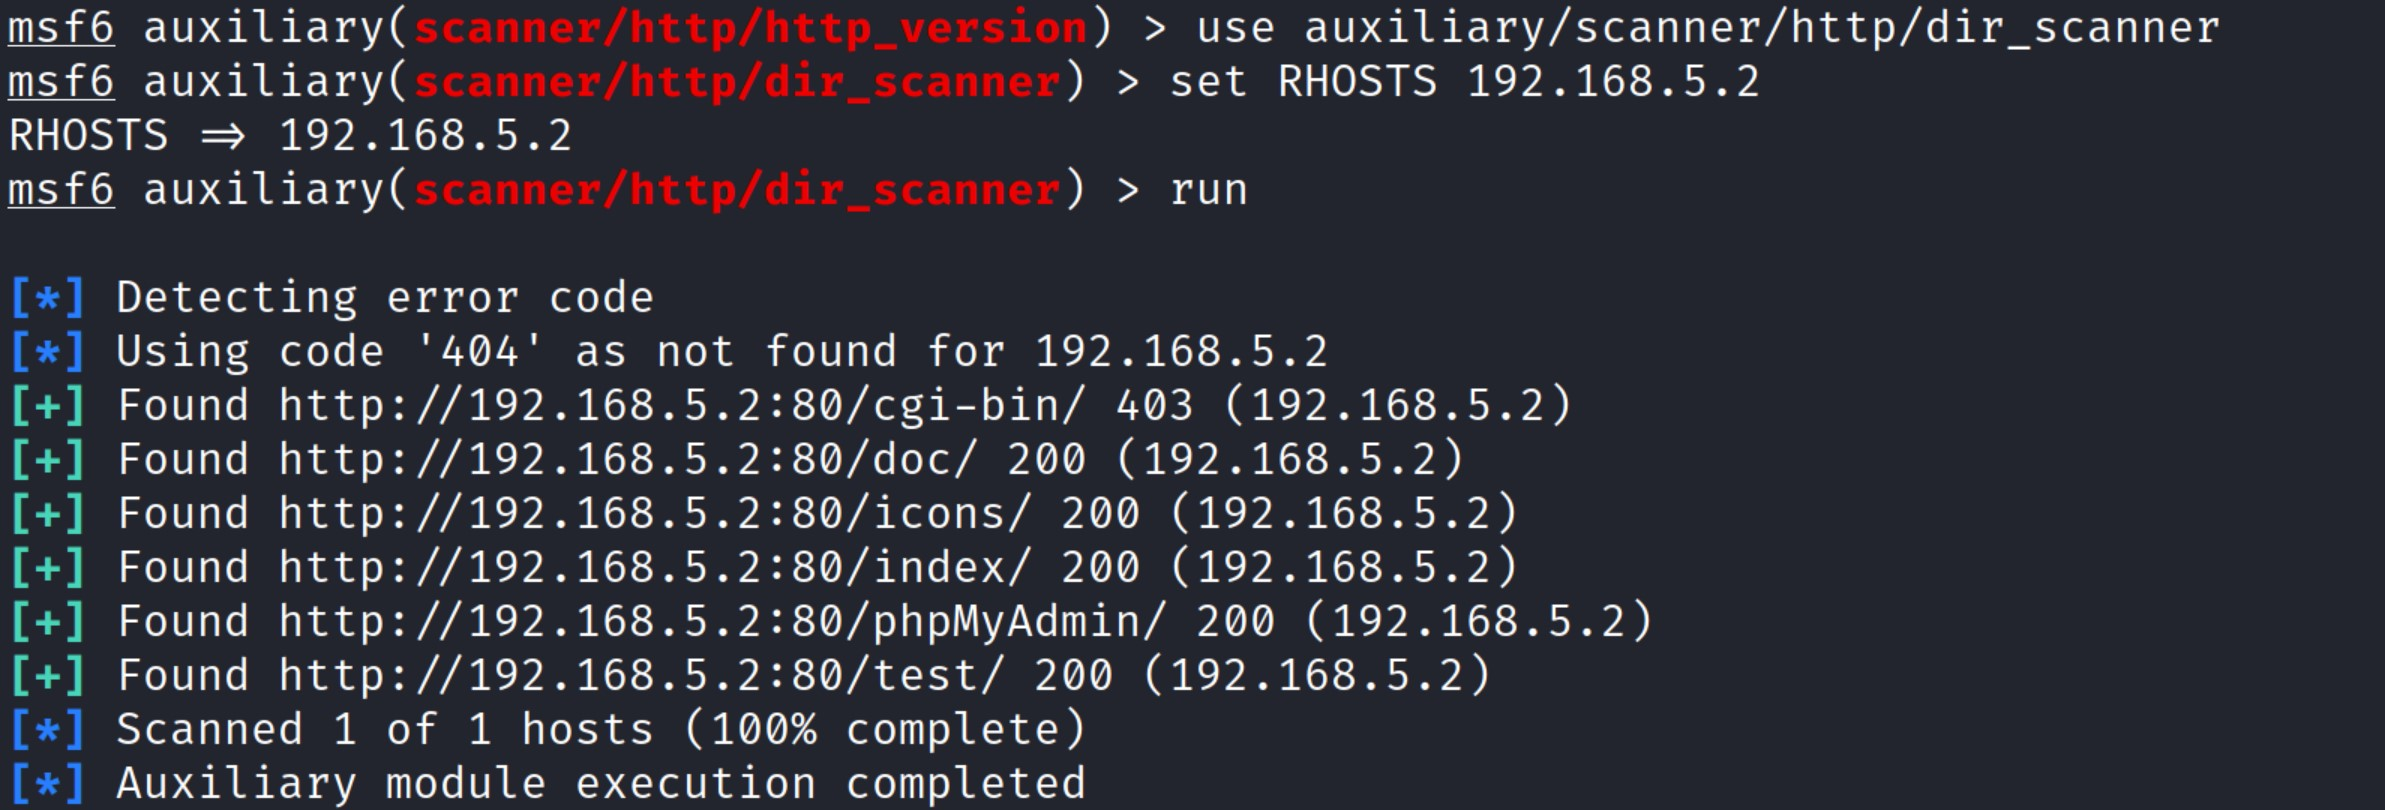
\includegraphics[width=\textwidth]{../drawable/exercise_1_screenshots/es1-httpdir.jpg}
	\caption{Scanning the HTTP version of a webserver and open directories}
	\label{fig:ex1:http}
\end{figure}

Figure \ref{fig:ex1:http} shows the output of both commands. We can observe how in the first case, we have an Apache web server running on top of a very insecure \texttt{PHP 5.2.4}, open on port \texttt{80}. This will be a very tasty target later on. To add insult to injury, a lot of directories are left exposed on the server, including the \texttt{phpMyAdmin} folder.

During the scan, it may be noticed that the scanner isn't exactly as quick as we would expect. This is because Metasploit allows customization of the number of concurrent threads (and therefore open connections) allowed during a scan. We can fix this by setting the \texttt{THREADS} variable. A value such as 50 is perfectly reasonable in a Linux environment such as ours. 

If we were,for example to launch a scan on the DISI website and its subnet (\texttt{disi.unitn.it/24}), we could see the sheer amount of tracked webservers and imagine how long it would take to scan all of them with a single thread. Figure \ref{fig:ex1:http-disi} shows a small snippet of an ongoing scan against that subnet.

\begin{figure}[htbp]
	\centering
	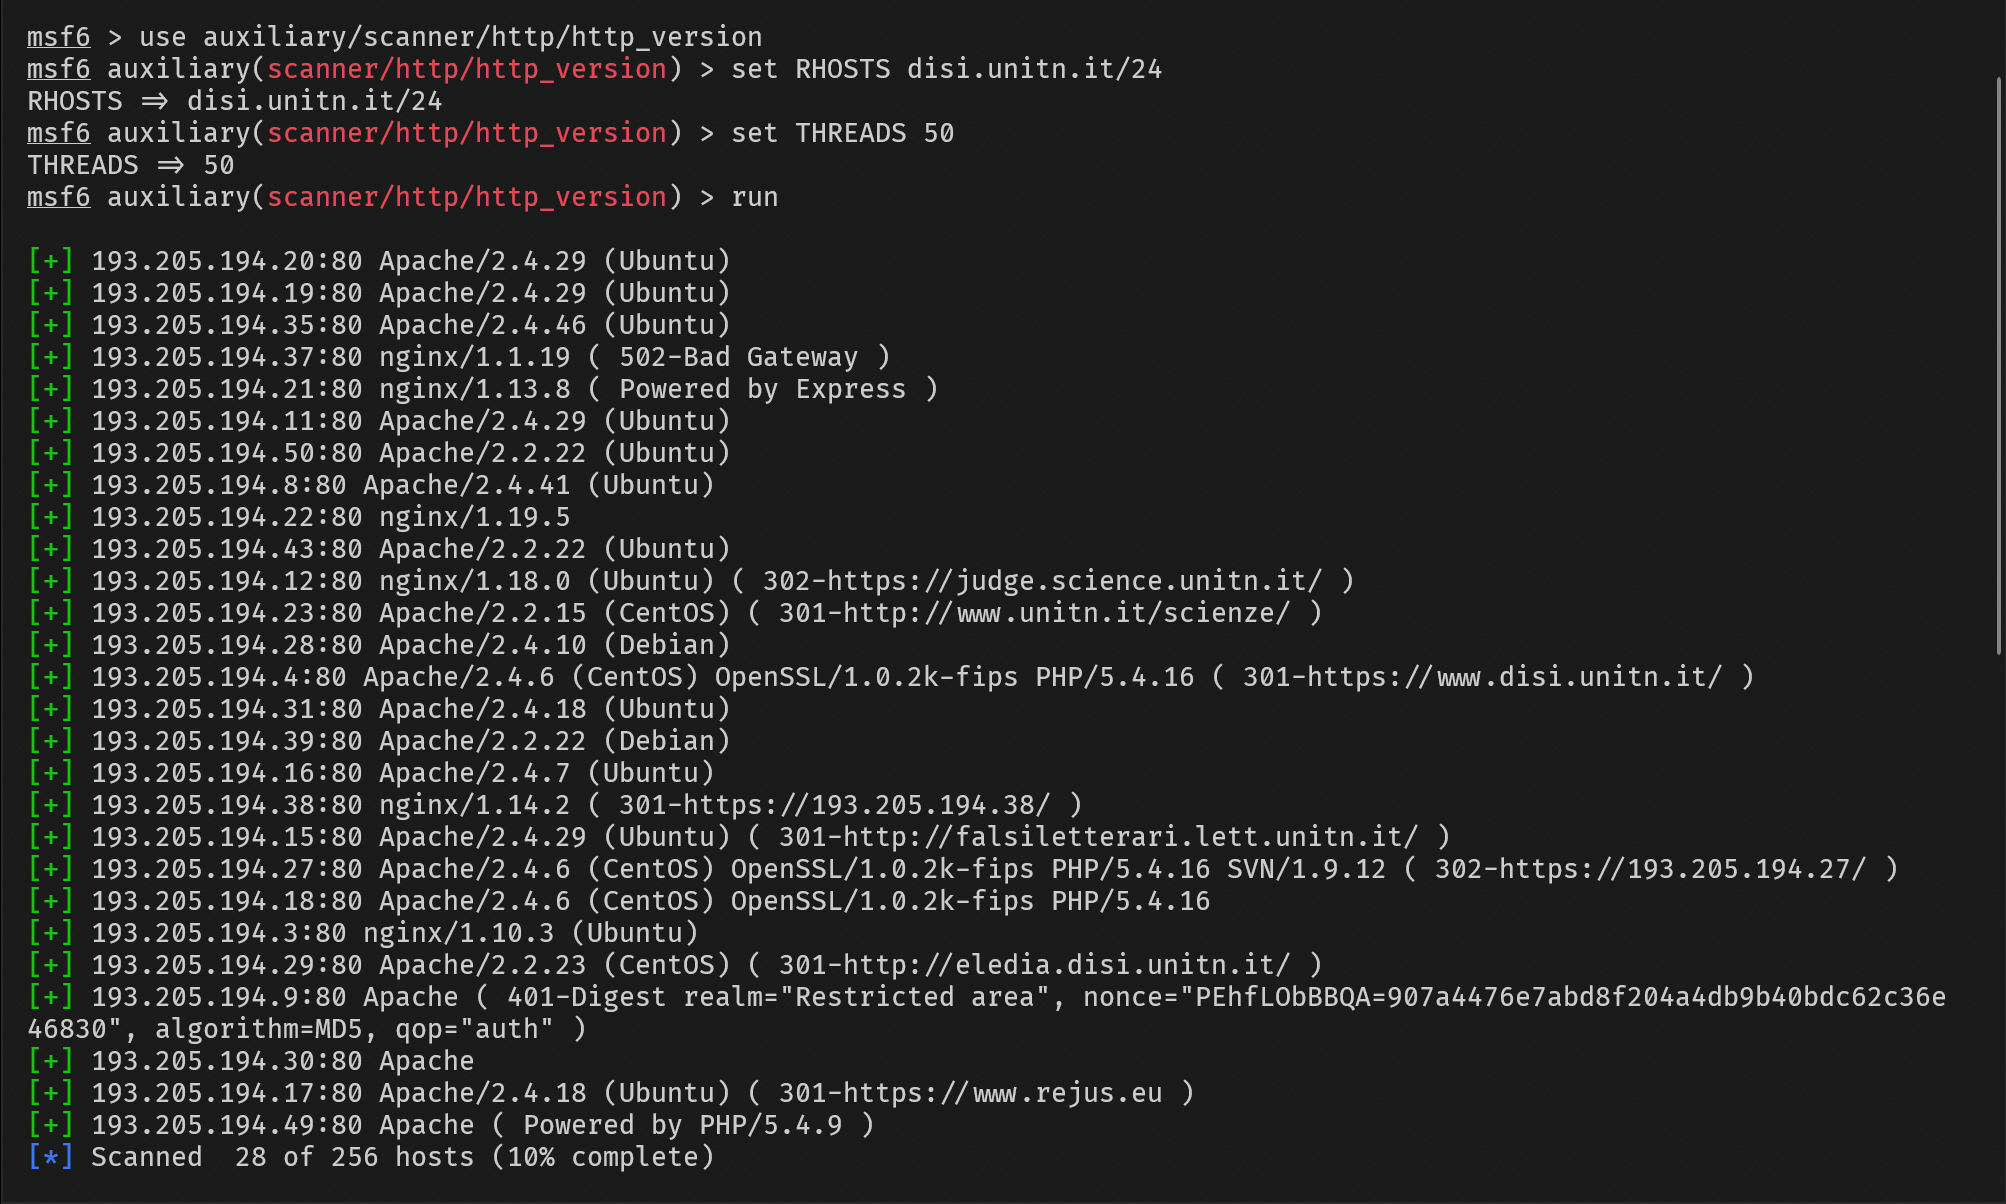
\includegraphics[width=0.85\textwidth]{../drawable/exercise_1_screenshots/es1-http-disi.png}
	\caption{Scanning the HTTP versions of the \texttt{disi.unitn.it} subnet}
	\label{fig:ex1:http-disi}
\end{figure}

This concludes the first exercise. We are now ready for a full fledged exploit against a slightly more advanced target.

\clearpage
\section{Exercise 2}
\label{sec:ex2}

We can now take a first look at Metasploit's exploit modules. Let us start from scratch, pretending Exercise 1 was never done and requiring a new scan.

\subsection{Setting up the database}
\label{subsec:ex2:setting-up-db}

In order to look at the services offered by the target machine - which will again be Metasploitable - we are now going to use \texttt{Nmap} instead of the auxiliary modules.

To get started with Metasploit's integration with Nmap, we need to verify that the database is alive and working. For the \texttt{ova} installation, this should be almost guaranteed. For the installation from scratch, please double check before proceeding. Figure \ref{fig:ex2:db_status} shows the correct output of \hltexttt{db\_status}.

\begin{figure}[htbp]
    \centering
    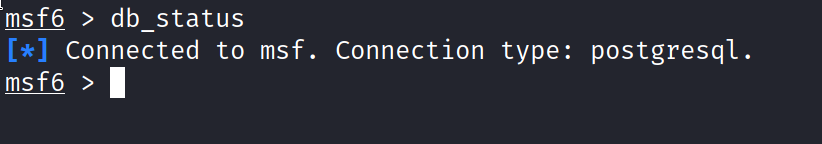
\includegraphics[width=0.5\textwidth]{../drawable/exercise_2_screenshots/db_status.png}
    \caption{Checking the DB setup is alive and working}
    \label{fig:ex2:db_status}
\end{figure}

The database is divided into \textit{workspaces}, which allow segmenting of the data stored inside. With \hltexttt{\mbox{workspace}} command, workspaces can be created, switched, and destroyed. In this lab, we will just use the default workspace.

By using commands such as \hltexttt{hosts}, and \hltexttt{\mbox{services}}, we realise that having had the database on all the time actually already filled it up with information with previous scans (Figure \ref{fig:ex2:services_hosts}). If needed, it can be discarded with we can wipe data with \hltexttt{\mbox{hosts -d}} and \hltexttt{\mbox{services -d}}. Additionally, we can stop the previous connections with \hltexttt{\mbox{sessions -K}}.

\begin{figure}[htbp]
	    \centering
	    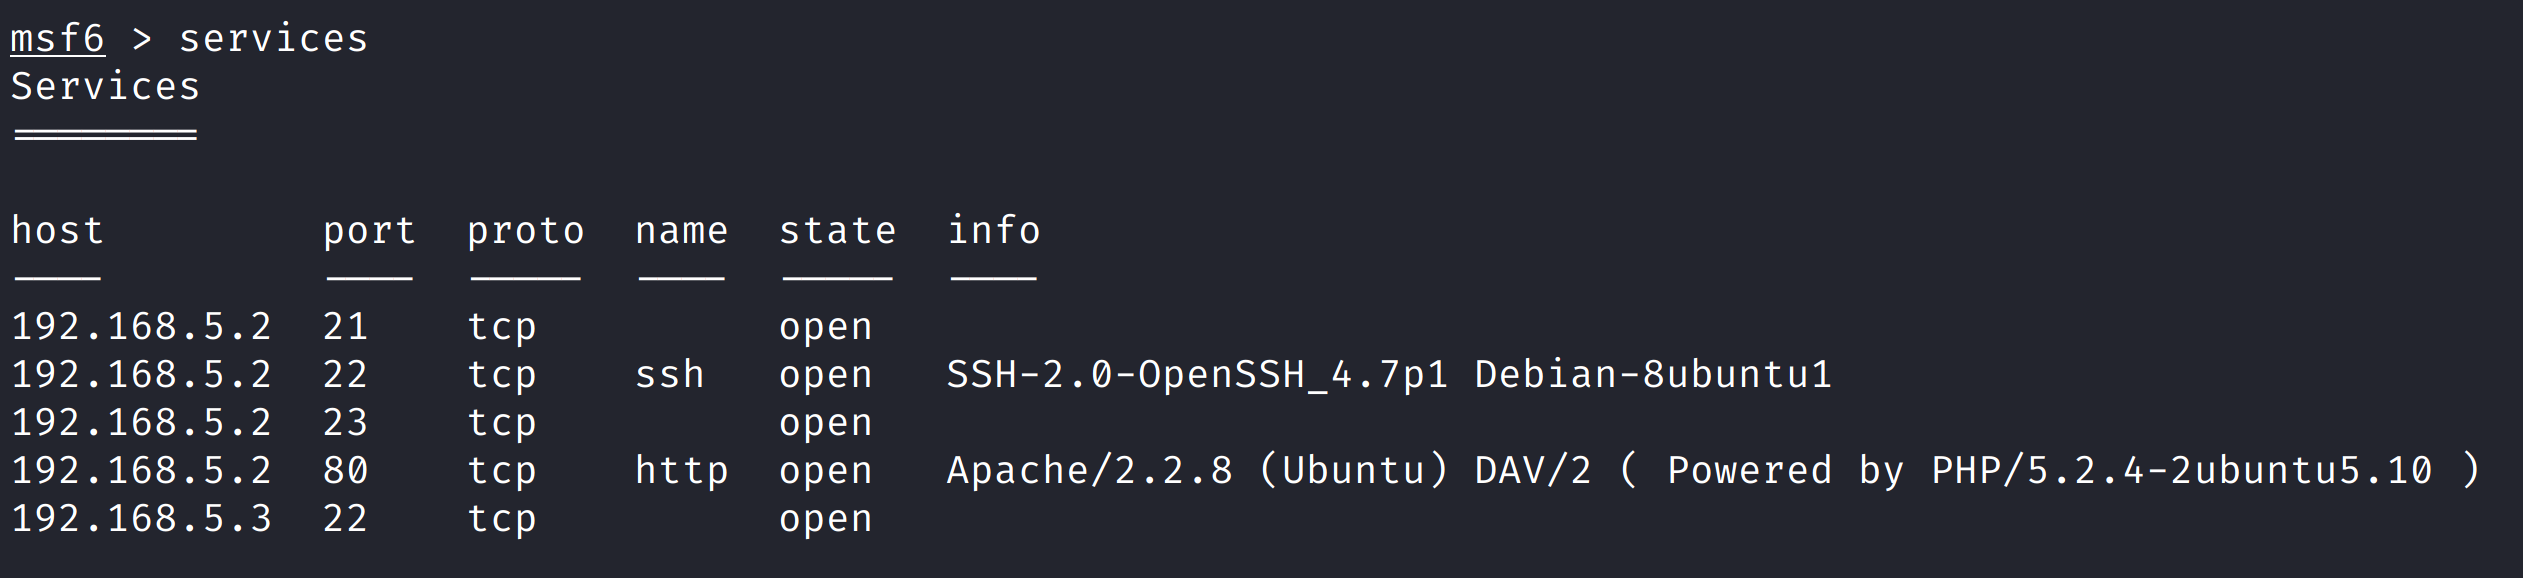
\includegraphics[width=0.6\textwidth]{../drawable/exercise_2_screenshots/services_before.png}
	    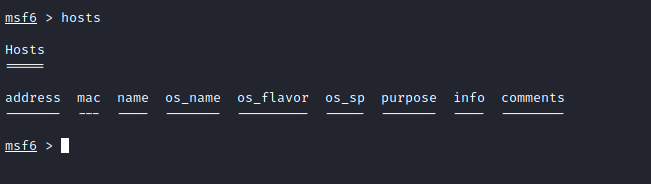
\includegraphics[width=0.6\textwidth]{../drawable/exercise_2_screenshots/hosts_empty.png}
	    \caption{\hltexttt{\mbox{services}} and \hltexttt{hosts}}
    \label{fig:ex2:services_hosts}
\end{figure}

\subsection{Scanning again}
\label{subsec:ex2:scanning-again}

We are now ready to scan. We begin by using \hltexttt{\mbox{db\_nmap}}. Its syntax is equivalent to that of \texttt{nmap}. In this case, we're going to inspect the Metasploitable machine at the 1000 most popular ports (the list being provided by the tool) with a \texttt{TCP} scan. Additionally, we supply the \texttt{-O} flag, which instructs \texttt{db\_nmap} to perform OS fingerprinting.

\begin{lstlisting}
db_nmap --top-ports 1000 192.168.5.2-3 -O
\end{lstlisting}

Other types of scan are outside the scope of this laboratory, and can be found at the official \texttt{Nmap} website\footnote{https://nmap.org/docs.html}. Figure \ref{fig:ex2:db_nmap} shows the output of the command.

\begin{figure}[htbp]
    \centering
    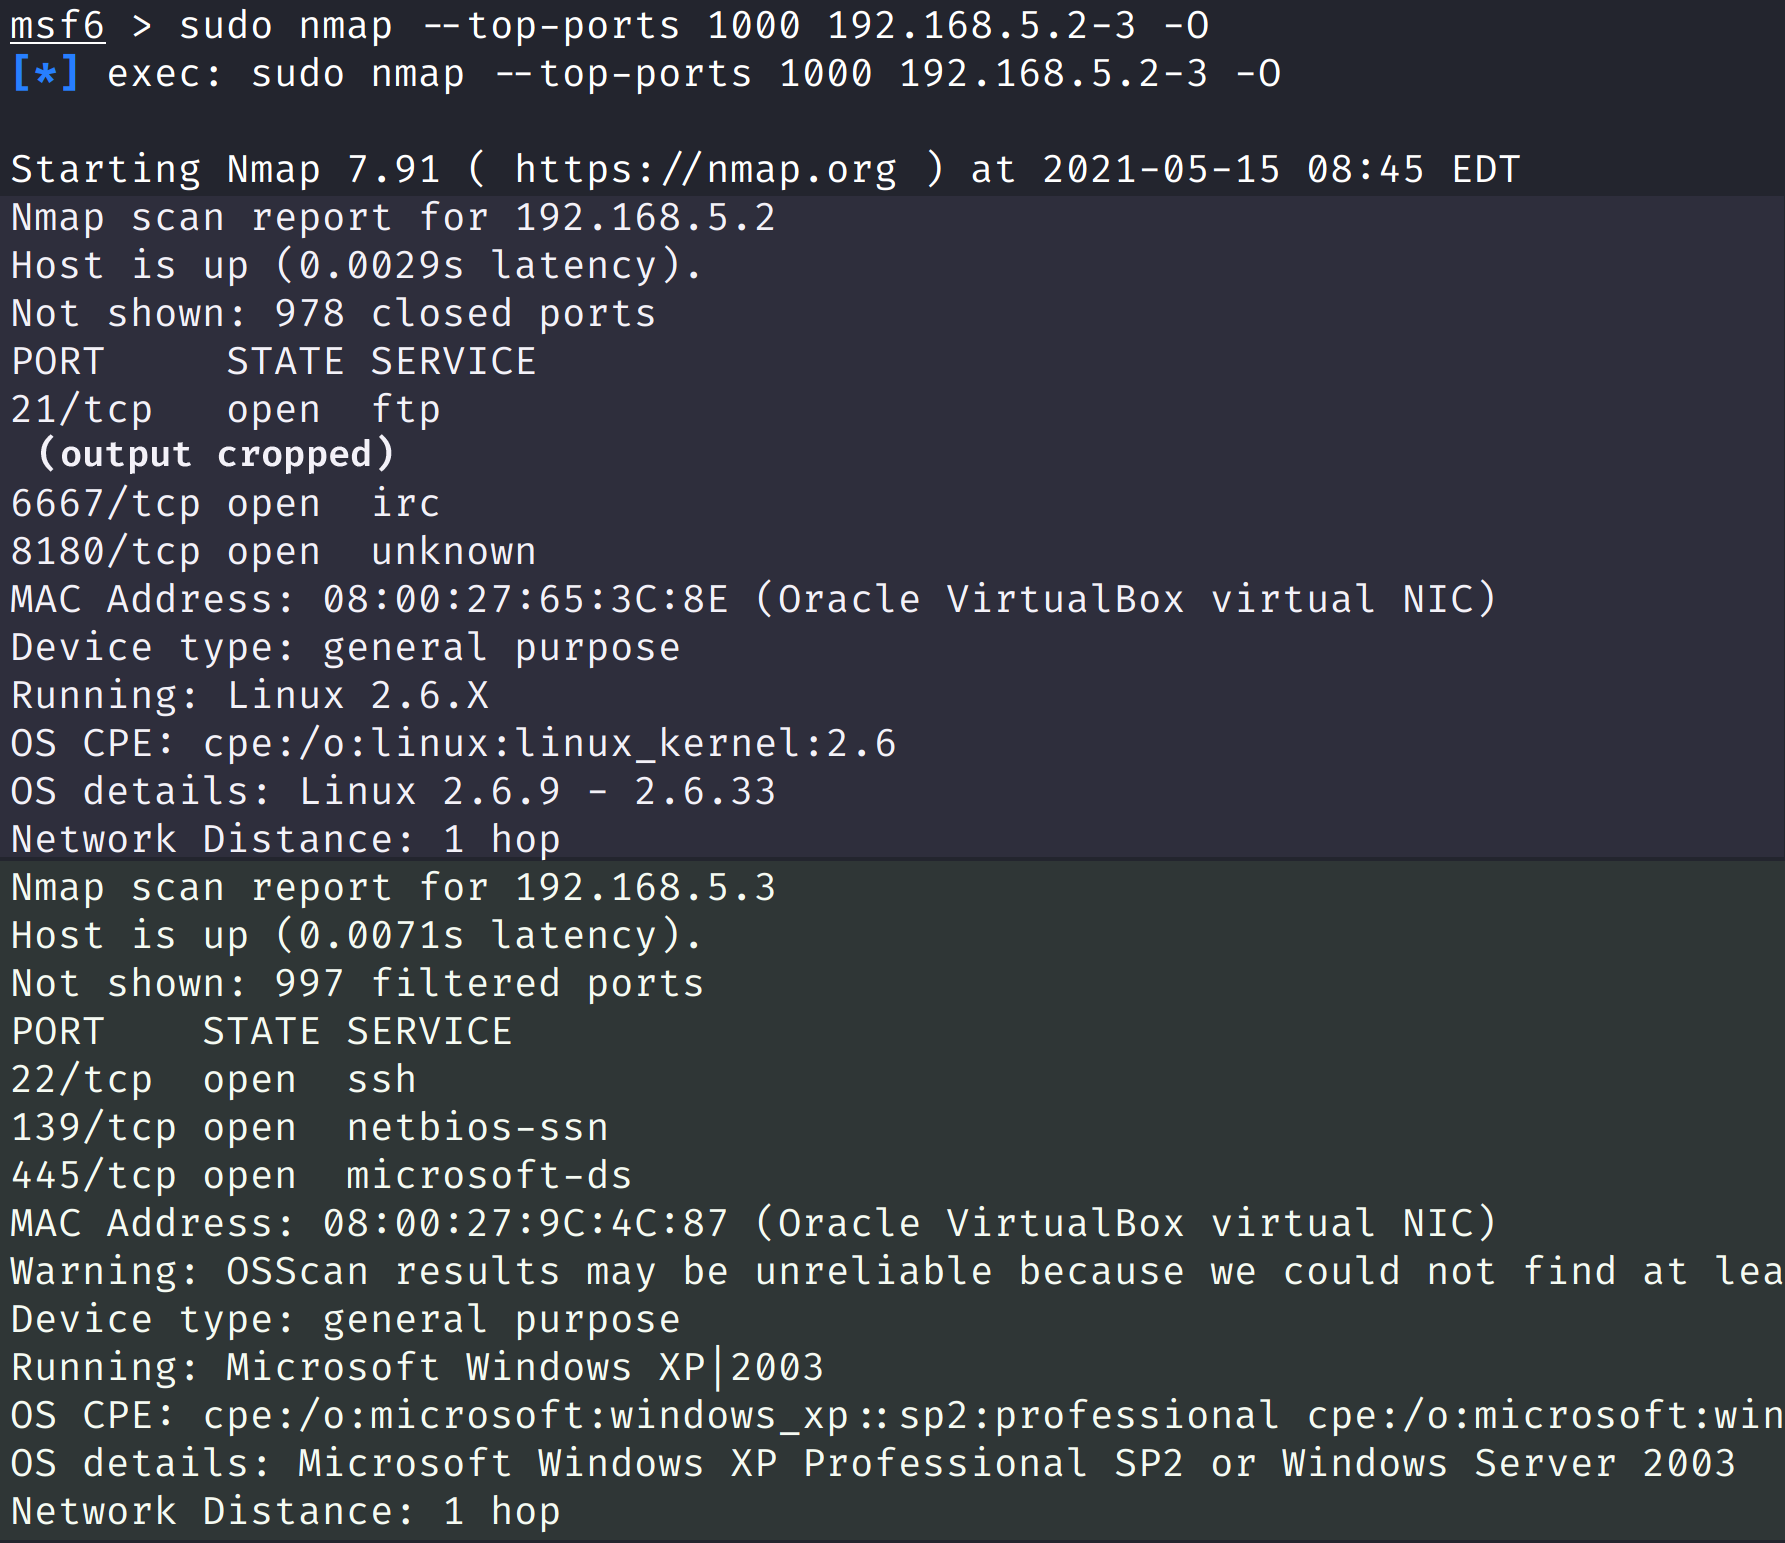
\includegraphics[width=0.8\textwidth]{../drawable/exercise_2_screenshots/db_nmap_v2.png}
    \caption{Scanning the potential victims}
    \label{fig:ex2:db_nmap}
\end{figure}

Now that the database is populated, we can check again \hltexttt{\mbox{services}}. We will notice that the table has been populated with the newly found services from our target. Figure \ref{fig:ex2:services_full_cropped} shows the output of the command.

\begin{figure}[htbp]
    \centering
    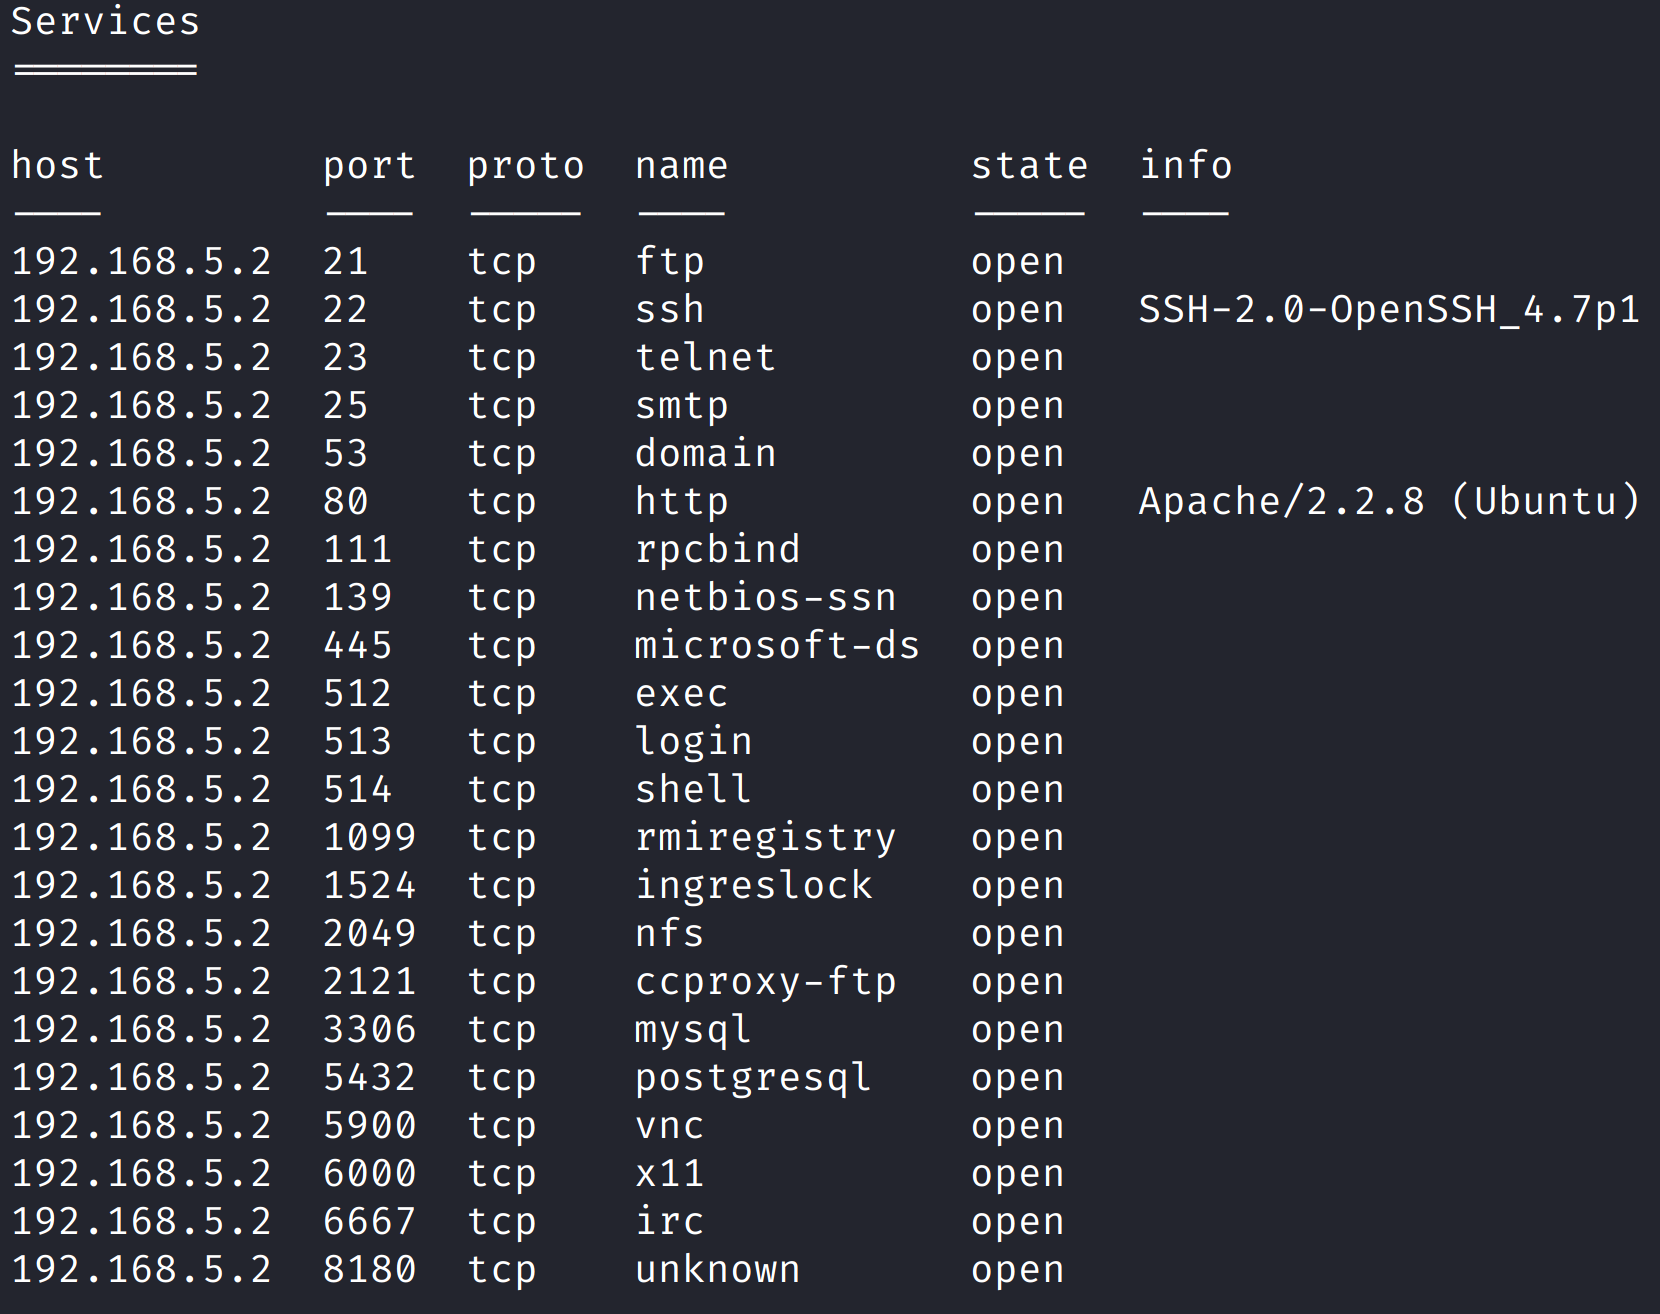
\includegraphics[width=0.7\textwidth]{../drawable/exercise_2_screenshots/services_full_v2.png}
    \caption{Checking the data that we gathered}
    \label{fig:ex2:services_full_cropped}
\end{figure}

From the previous exercise - and as \hltexttt{\mbox{services}} reminds us - the \texttt{HTTP} server on the Metasploitable machine is old and runs a vulnerable version of \texttt{PHP}. However, this time we're not going to slip this through unnoticed.

%As we did in the previous exercise, we can now use a scanner to get some more details on the HTTP service:

%\begin{lstlisting}
%use auxiliary/scanner/http/http_version
%\end{lstlisting}

%Figure \ref{fig:ex2:use_http_version_scanner+execute_http_version} shows the output of the command.

%\begin{figure}[htbp]
%    \centering
%    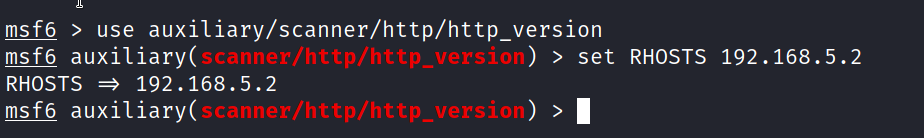
\includegraphics[width=\textwidth]{../drawable/exercise_2_screenshots/use_http_version_scanner.png}
%    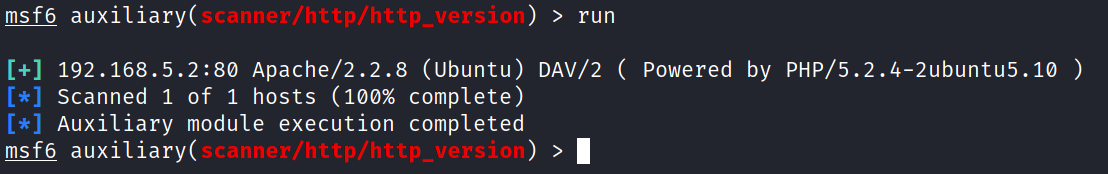
\includegraphics[width=\textwidth]{../drawable/exercise_2_screenshots/execute_http_version.png}
%    \caption{Preparing the scanner, and then hitting \hltexttt{run}}
%    \label{fig:ex2:use_http_version_scanner+execute_http_version}
%\end{figure}

% Of course, the results aren't surprising: the web server is highly vulnerable. 

\subsection{Taking the knives out}
\label{subsec:ex2:taking-knives-out}

We're now going to exploit the fact that this \texttt{PHP} version is riddlded with vulnerabilities\footnote{PHP doesn't exactly have a great record from a security standpoint: see\\\texttt{https://www.cvedetails.com/product/128/PHP-PHP.html?vendor\_id=74}}. 

At this point, we can go to the next phase and find a suitable exploit and payload for our vulnerability. A quick trip to a CVE database can yield tremendous results. For this laboratory, we decided to settle on \texttt{CVE-2012-1823}\footnote{\texttt{https://www.cvedetails.com/cve/CVE-2012-1823/}}. The vulnerability states the following:

\medskip

\begin{center}
\noindent\fbox{%
    \parbox{0.9\textwidth}{%
        \texttt{sapi/cgi/cgi\_main.c} in PHP before 5.3.12 and 5.4.x before 5.4.2, when configured as a CGI script (aka php\-cgi), does not properly handle query strings that lack an = (equals sign) character, which allows remote attackers to execute arbitrary code by placing command-line options in the query string, related to lack of skipping a certain php\_getopt for the 'd' case.
    }%
}
\end{center}

\medskip


{
\noindent
\begin{minipage}{\linewidth}

The following is a code snippet from \texttt{cgi\_main.c}, the source of the buffer overflow:

\begin{lstlisting}[showspaces=false,breaklines=true]
// [...] here len is the same length of php_optarg
memcpy(
    cgi_sapi_module.ini_entries + ini_entries_len,
    php_optarg,
    len
);
// [...]
\end{lstlisting}
\end{minipage}
}

{
\noindent
\begin{minipage}{\linewidth}

While this is another snippet from the exploit file.

\begin{lstlisting}
payload_oneline = "<?php " + payload.encoded.gsub(/\s*#.*$/, "").gsub("\n", "")
response = send_request_cgi( {
'method' => "POST",
'global' => true,
// [...]
}, 0.5)
\end{lstlisting}
\end{minipage}
}

Let us load up the exploit as usual.

\begin{lstlisting}
use exploit/multi/http/php_cgi_arg_injection
\end{lstlisting}

Then, we \hltexttt{set} our \texttt{RHOSTS} and \texttt{LHOST} variables. Figure \ref{fig:ex2:use_exploit_cgi_exception+set_exploit_options} shows these two steps. Notice how now the default payload defaults to \texttt{php/meterpreter/reverse\_tcp}.

\begin{figure}[htbp]
    \centering
    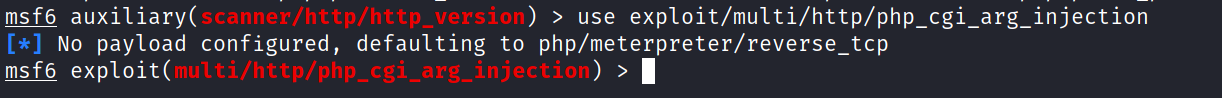
\includegraphics[width=0.8\textwidth]{../drawable/exercise_2_screenshots/use_exploit_cgi_exception.png}
    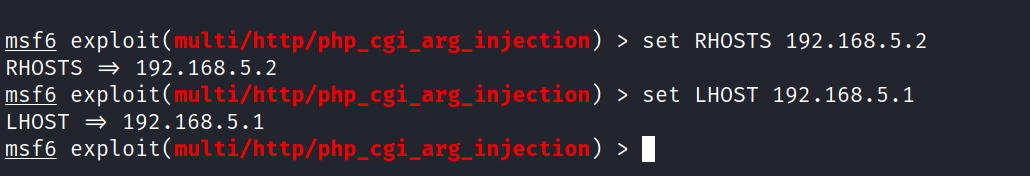
\includegraphics[width=0.8\textwidth]{../drawable/exercise_2_screenshots/set_exploit_options.png}
    \caption{Using the default payload and setting options}
    \label{fig:ex2:use_exploit_cgi_exception+set_exploit_options}
\end{figure}

As we said before, the payloads in Metasploit are highly configurable, and each one of them may provide advantadges or disadvantages. For simplicity purposes, we decided to stick to the default one, which provides a \textit{reverse shell} with Meterpreter. Figure \ref{fig:ex2:shell_opened} shows what opening the shell actually looks like.

\begin{figure}[htbp]
    \centering
    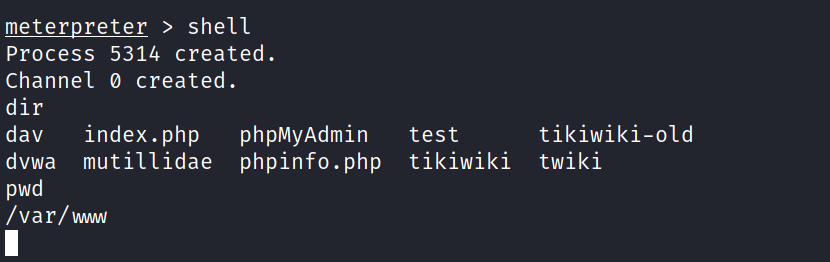
\includegraphics[width=0.7\textwidth]{../drawable/exercise_2_screenshots/shell_opened.png}
    \caption{Opening a shell with Meterpreter}
    \label{fig:ex2:shell_opened}
\end{figure}

To end the exercise, we provide a little insight on what the payload actually provided. Once the exploit has been run on the target, we theoretically have the capability to \textit{execute arbitrary code by placing command-line options in the query string}, as the CVE definition says. This is the perfect moment for executing a payload's arbitrary code, and where our Meterpreter comes into play.

Meterpreter is a dynamically extensible payload that uses in-memory DLL injection stagers and is extended over the network at runtime. 
It communicates over the stager socket and provides a comprehensive client-side Ruby API. It features command history, tab completion, channels, and more.\cite{online:meterpreter} In this case, Meterpreter was installed using a reverse shell: a shell that was initiated by the victim - unknowingly - rather than from the attacker. Figure \ref{fig:ex2:schema_reverse_shell} shows a diagram representing the logical idea behind reverse shells.

\begin{figure}[htbp]
    \centering
    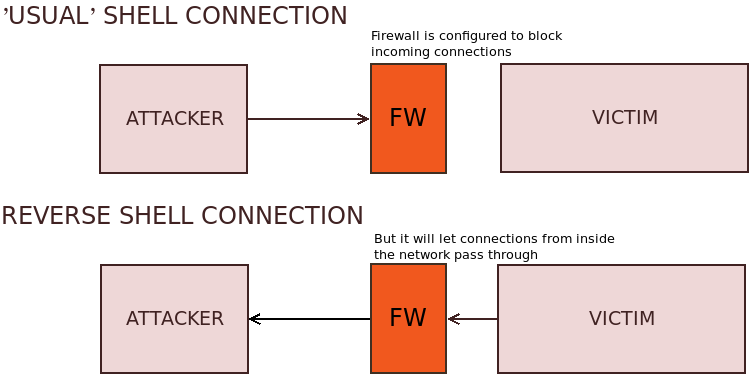
\includegraphics[width=0.7\textwidth]{../drawable/decorations/schema_reverse_shell.png}
    \caption{Shell and reverse shell connections}
    \label{fig:ex2:schema_reverse_shell}
\end{figure}

The exercise has finished: for the final one, we're going even deeper on Metasploit, spicing things up with the usage of PDF files.

\clearpage
\section{Exercise 3}
\label{sec:ex3}
For the third exercise, we are going to exploit another buffer overflow vulnerability, this time with version \texttt{9.0} of Adobe Reader. We introduce the concept of process migration of the remote shell code, making the exploit execution less visible to the victim.

In order to carry out this attack, we are going to focus on our Windows XP SP2 machine. While at a first glance this might seem like an extremely outdated and pointless attack, in reality \texttt{PDF} files are often the veichle of exploits, even in 2021\footnote{\url{https://threatpost.com/adobe-zero-day-bug-acrobat-reader/166044/}}. First, we will craft our malicious \texttt{PDF} using Metasploit and bundle it into an apparently innocuous file. Then, we will deliver the payload to the target's machine. By the time the victim has opened the file and closed Adobe Reader, we will have full control of his machine.

\subsection{Infected \texttt{PDF} file creation}
\label{subsec:ex3:infected-pdf-file-creation}
The initial phase of the attack in completely handled by \hltexttt{\mbox{msfconsole}}. A set of \hltexttt{\mbox{msfconsole}} scripts are dedicated to the generation of corrupted files, under \texttt{exploit/windows/fileformat/}. This time, we're going to use the \texttt{adobe\_jbig2decode} (Figure \ref{fig:ex3:selecting-exploit}).

\begin{figure}[htbp]
    \centering
    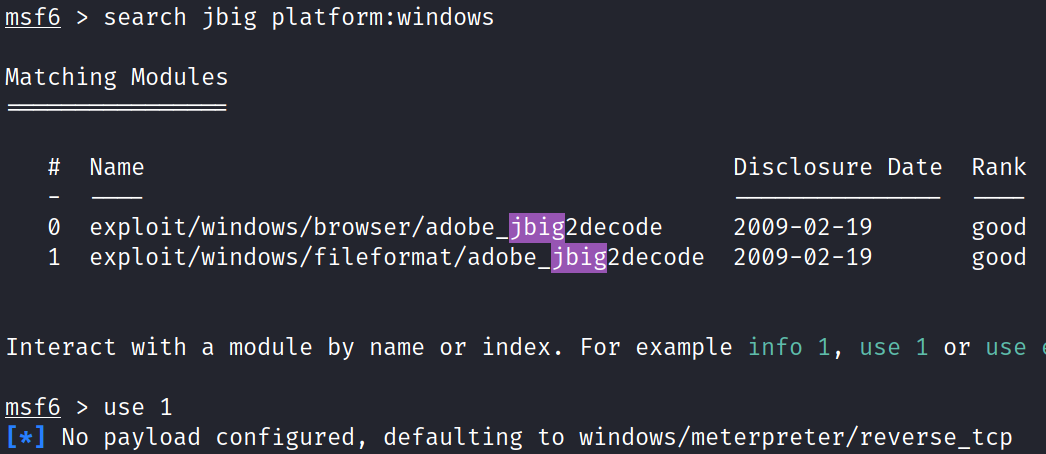
\includegraphics[width=0.7\textwidth]{../drawable/exercise_3_screenshots/module_selection.png}
    \caption{Selecting the exploit to use}
    \label{fig:ex3:selecting-exploit}
\end{figure}

The payload for the infected file will create a reverse shell from the specified host. We set the \texttt{LHOST} and \texttt{LPORT} parameters for binding the shell, and we create the file (Figure \ref{fig:ex3:running-exploit}).

\begin{figure}[htbp]
    \centering
    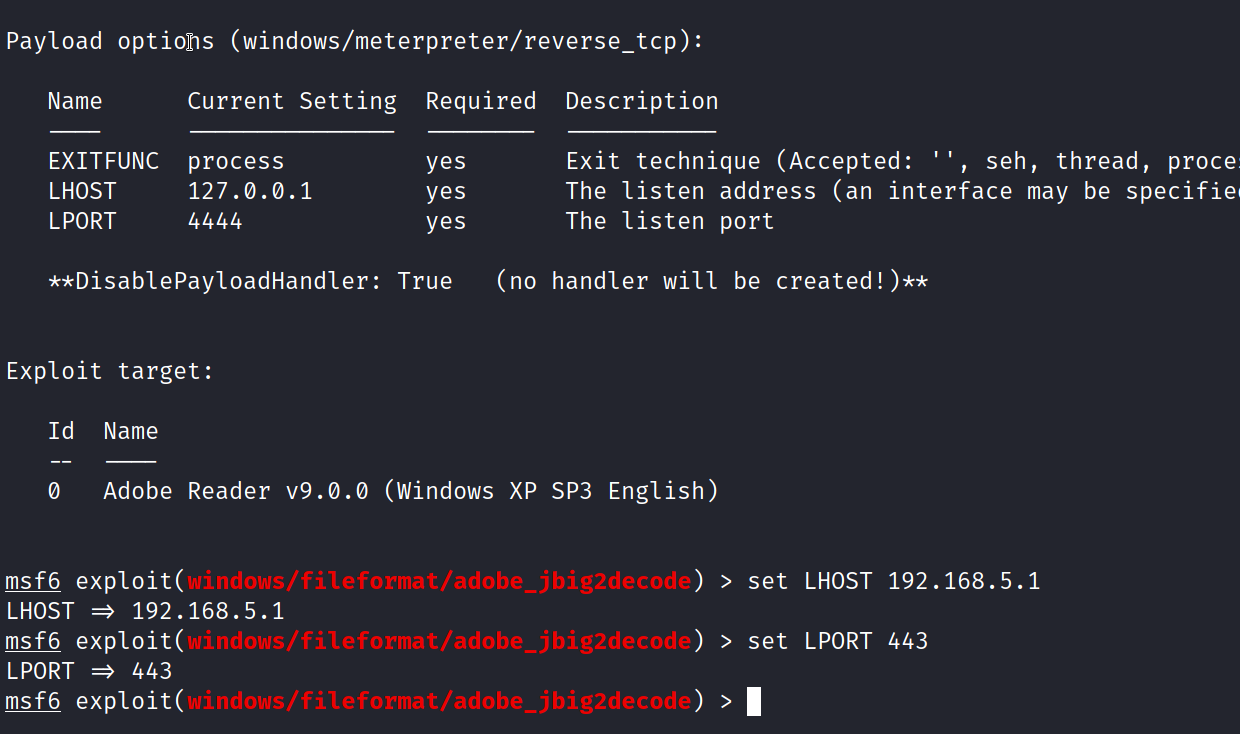
\includegraphics[width=0.7\textwidth]{../drawable/exercise_3_screenshots/module_set_options.png}
    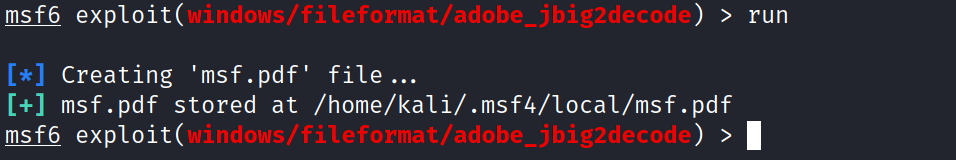
\includegraphics[width=0.7\textwidth]{../drawable/exercise_3_screenshots/run_exploit.png}
    \caption{Setting the options and generating the infected \texttt{PDF}}
    \label{fig:ex3:running-exploit}
\end{figure}

\subsection{Simulated infection}
\label{subsec:ex3:simulated-infection}

In a real life situation, the file could be sent to the victim via email or using a removable media. This is a perfect example on how social engineering could be exploited in conjunction with code-based hacking in order to get even larger footholds in target networks. Moreover, it sends red flags to pentesters who must take care of both automated and well-crafted attacks to the network in their reports.
\begin{figure}[htbp]
    \centering
    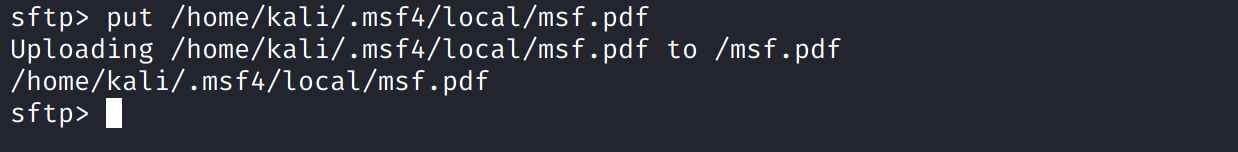
\includegraphics[width=0.7\textwidth]{../drawable/exercise_3_screenshots/put_completed.png}
    \caption{Sending the file to our Windows XP VM}
    \label{fig:ex3:sending-file}
\end{figure}

In this simulation, the file is copied to the victim via \texttt{SFTP}, since in this exercise we are more interested in the effects of the exploit rather than the delivery of the infected file. Figure \ref{fig:ex3:sending-file} shows the sending of the file. Notice that an \texttt{SFTP} server was previously installed on the Windows XP machine, listening on port \texttt{22}, as \texttt{SFTP} runs on the \texttt{SSH} port instead of the regular \texttt{FTP} ones. That port was the only one appearing as open in the results of the scans in Sections \ref{sec:exercise1:tcpscanning} and \ref{subsec:ex2:scanning-again}.

\subsection{Reverse shell handler}
\label{subsec:ex3:reverse-shell-handler}

Differently from the previous exercise, the reverse shell handler needs to be started manually (Figure \ref{fig:ex3:reverse-shell-handler}). This is because the previous exploit was "just" limited to the creation of the malicious file and did not provide an automatic connection feature. However, we can quickly take care of this problem.

\begin{figure}[htbp]
    \centering
    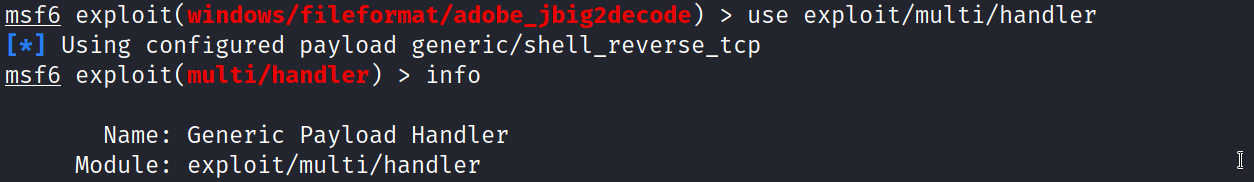
\includegraphics[width=0.7\textwidth]{../drawable/exercise_3_screenshots/generic_payload_handler.png}
    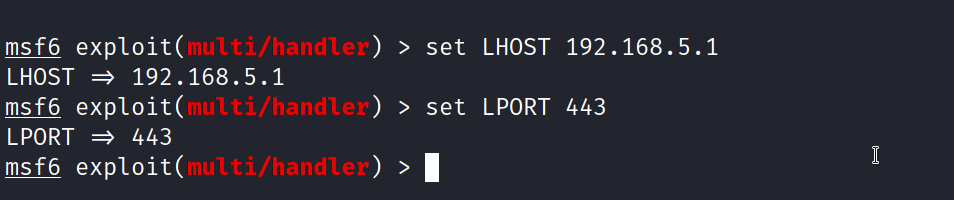
\includegraphics[width=0.7\textwidth]{../drawable/exercise_3_screenshots/set_handler_parameters.png}
    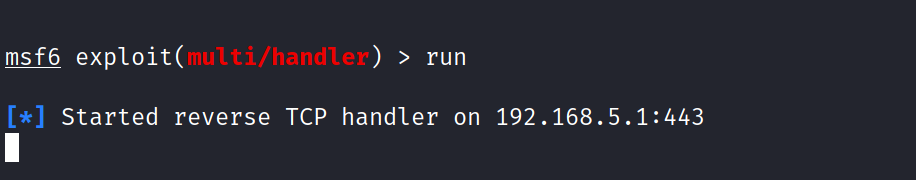
\includegraphics[width=0.7\textwidth]{../drawable/exercise_3_screenshots/handler_listening.png}
    \caption{Starting the reverse shell handler}
    \label{fig:ex3:reverse-shell-handler}
\end{figure}

When the victim opens the \texttt{PDF} file, the exploit code causes a buffer overflow, and redirects the execution of the Adobe Reader process towards the code of our payload. The payload contacts the attacker on port \texttt{443} (port for \texttt{HTTPS} service); using well-known ports allows us to bypass the victim's host firewall. Figure \ref{fig:ex3:reverse-shell-opened} shows a successfully open shell.

\begin{figure}[htbp]
    \centering
    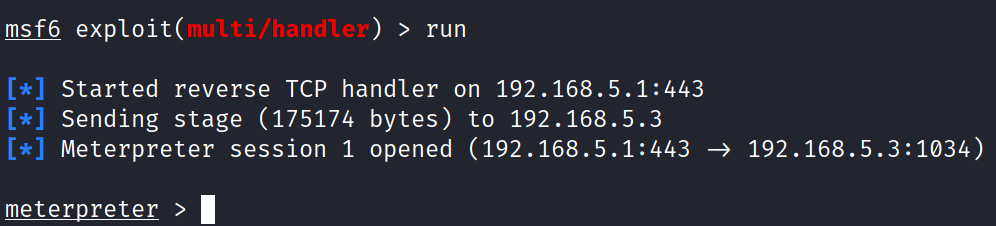
\includegraphics[width=0.7\textwidth]{../drawable/exercise_3_screenshots/meterpreter_opened.png}
    \caption{Reverse shell managed to reach the attacker}
    \label{fig:ex3:reverse-shell-opened}
\end{figure}

\subsection{Exploit code migration}
\label{subsec:ex3:exploit-code-migration}

After the victim has opened the file, Adobe Reader freezes. This may prompt the user to forcefully kill the viewer, thus terminating our reverse shell. To avoid this, we can use a standard functionality of the Meterpreter console to migrate the code of the reverse shell to another process. Figure \ref{fig:ex3:migrating-shell} shows this process.

\begin{figure}[htbp]
    \centering
    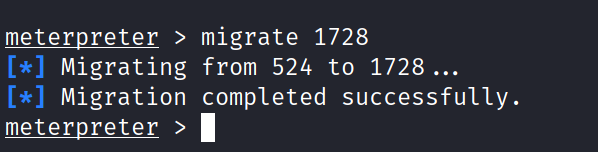
\includegraphics[width=0.7\textwidth]{../drawable/exercise_3_screenshots/meterpreter_migration.png}
    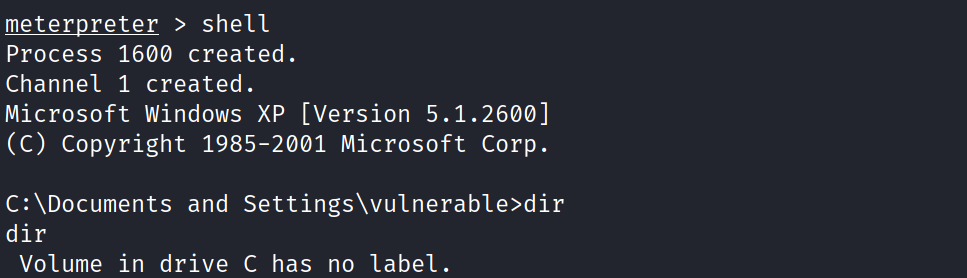
\includegraphics[width=0.7\textwidth]{../drawable/exercise_3_screenshots/meterpreter_shell_opened_cropped.png}
    \caption{Migrating shell code to another process}
    \label{fig:ex3:migrating-shell}
\end{figure}

This works because Windows allows to write data into a process memory, allowing to "hot patch" the code of a process with our exploit. When the migration completes, the reverse shell remains active even if the victim kills the Adobe Reader process.

\subsection{Exploit details}
\label{subsec:ex3:exploit-details}
 The exploit used in this exercise is \texttt{CVE-2009-0658}: 
\medskip
\begin{center}
\noindent\fbox{%
    \parbox{0.9\textwidth}{%
    Buffer overflow in Adobe Reader 9.0 and earlier, and Acrobat 9.0 and earlier, allows remote attackers to execute arbitrary code via a crafted \texttt{PDF} document, related to a non-JavaScript function call and possibly an embedded JBIG2 image stream, as exploited in the wild in February 2009 by \texttt{Trojan.Pidief.E}.        
    }%
}
\end{center}
\medskip

The attack is not completely invisible to the target. Tools like \texttt{netstat} can see the connection towards the attacker. Depending on the situation, the user may or may not be capable of using such tools during their daily work usage. Either way, targeting a less tech savy user would be the wisest choice here.

\begin{figure}[htbp]
    \centering
    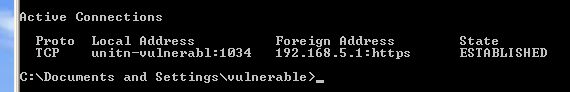
\includegraphics[width=0.75\textwidth]{../drawable/exercise_3_screenshots/victim_connection.PNG}
    \caption{Output of \texttt{netstat} on victim machine while the payload executes}
    \label{fig:ex3:victim-connections}
\end{figure}

\clearpage

\endgroup

\addcontentsline{toc}{section}{References}

\bibliographystyle{IEEEtran-sorted-tt}
\bibliography{biblio}

\end{document}
